% Options for packages loaded elsewhere
\PassOptionsToPackage{unicode}{hyperref}
\PassOptionsToPackage{hyphens}{url}
\PassOptionsToPackage{dvipsnames,svgnames*,x11names*}{xcolor}
%
\documentclass[
  11pt,
]{book}
\usepackage{lmodern}
\usepackage{amssymb,amsmath}
\usepackage{ifxetex,ifluatex}
\ifnum 0\ifxetex 1\fi\ifluatex 1\fi=0 % if pdftex
  \usepackage[T1]{fontenc}
  \usepackage[utf8]{inputenc}
  \usepackage{textcomp} % provide euro and other symbols
\else % if luatex or xetex
  \usepackage{unicode-math}
  \defaultfontfeatures{Scale=MatchLowercase}
  \defaultfontfeatures[\rmfamily]{Ligatures=TeX,Scale=1}
\fi
% Use upquote if available, for straight quotes in verbatim environments
\IfFileExists{upquote.sty}{\usepackage{upquote}}{}
\IfFileExists{microtype.sty}{% use microtype if available
  \usepackage[]{microtype}
  \UseMicrotypeSet[protrusion]{basicmath} % disable protrusion for tt fonts
}{}
\makeatletter
\@ifundefined{KOMAClassName}{% if non-KOMA class
  \IfFileExists{parskip.sty}{%
    \usepackage{parskip}
  }{% else
    \setlength{\parindent}{0pt}
    \setlength{\parskip}{6pt plus 2pt minus 1pt}}
}{% if KOMA class
  \KOMAoptions{parskip=half}}
\makeatother
\usepackage{xcolor}
\IfFileExists{xurl.sty}{\usepackage{xurl}}{} % add URL line breaks if available
\IfFileExists{bookmark.sty}{\usepackage{bookmark}}{\usepackage{hyperref}}
\hypersetup{
  pdftitle={Dispense sul disegno sperimentiale},
  pdfauthor={Giorgio Marrubini e Camillo Melzi},
  colorlinks=true,
  linkcolor=Maroon,
  filecolor=Maroon,
  citecolor=Blue,
  urlcolor=Blue,
  pdfcreator={LaTeX via pandoc}}
\urlstyle{same} % disable monospaced font for URLs
\usepackage[left=2cm, right=2.5cm, top=2.5cm, bottom=2.5cm]{geometry}
\usepackage{longtable,booktabs}
% Correct order of tables after \paragraph or \subparagraph
\usepackage{etoolbox}
\makeatletter
\patchcmd\longtable{\par}{\if@noskipsec\mbox{}\fi\par}{}{}
\makeatother
% Allow footnotes in longtable head/foot
\IfFileExists{footnotehyper.sty}{\usepackage{footnotehyper}}{\usepackage{footnote}}
\makesavenoteenv{longtable}
\usepackage{graphicx}
\makeatletter
\def\maxwidth{\ifdim\Gin@nat@width>\linewidth\linewidth\else\Gin@nat@width\fi}
\def\maxheight{\ifdim\Gin@nat@height>\textheight\textheight\else\Gin@nat@height\fi}
\makeatother
% Scale images if necessary, so that they will not overflow the page
% margins by default, and it is still possible to overwrite the defaults
% using explicit options in \includegraphics[width, height, ...]{}
\setkeys{Gin}{width=\maxwidth,height=\maxheight,keepaspectratio}
% Set default figure placement to htbp
\makeatletter
\def\fps@figure{htbp}
\makeatother
\setlength{\emergencystretch}{3em} % prevent overfull lines
\providecommand{\tightlist}{%
  \setlength{\itemsep}{0pt}\setlength{\parskip}{0pt}}
\setcounter{secnumdepth}{5}
\usepackage{booktabs}
\usepackage{amsmath}
\usepackage[italian]{babel}\addto\extrasitalian{
  \def\figureautorefname{Figura}
  \def\chapterautorefname{Capitolo}
  \def\sectionautorefname{Paragrafo}
  \def\subsectionautorefname{Paragrafo}
  \def\subsubsectionautorefname{Paragrafo}
  \def\equationautorefname{Equazione}
  \def\tableautorefname{Tabella}}
\usepackage{arydshln}
\usepackage[]{natbib}
\bibliographystyle{plainnat}

\title{Dispense sul disegno sperimentiale}
\author{Giorgio Marrubini e Camillo Melzi}
\date{}

\begin{document}
\maketitle

{
\hypersetup{linkcolor=}
\setcounter{tocdepth}{1}
\tableofcontents
}
\hypertarget{section}{%
\chapter*{}\label{section}}
\addcontentsline{toc}{chapter}{}

\hypertarget{glossario}{%
\chapter*{Glossario minimo}\label{glossario}}
\addcontentsline{toc}{chapter}{Glossario minimo}

Le voci seguenti sono in ordine alfabetico e riportano alcune definizioni di termini e concetti di base che ricorrono nelle dispense.
Le definizioni sono tratte dai riferimenti citati in bibliografia.
\citep{legarzantine2014, everittb.s.skrondala.2010, wonnacottt.h.wonnacottr.j.2002}

\textbf{Aleatorio, campione a., evento a., intervallo a., variabile a.}\\
Il termine aleatorio è sinonimo di casuale.
Deriva da ``alea'' che in latino significa dado.
Quindi aleatorio è aggettivo di un campione, un evento o altro la cui natura è legata al caso (v. anche la voce \emph{caso, casuale}).

\textbf{Analisi di correlazione}\\
Verifica del fatto che due variabili siano correlate tra loro.
V. \emph{Correlazione}.

\textbf{Analisi di regressione}\\
Definizione del modello funzionale per cui una proprietà Y dipende da un fattore X e quindi che valga la relazione Y = f(X).
Nel caso di più fattori, X\textsubscript{1}, X\textsubscript{2}, \ldots, X\textsubscript{n}, si parla di regressione multipla e si verifica quindi la validità della relazione Y = f(X\textsubscript{1}, X\textsubscript{2}, \ldots, X\textsubscript{n}).

\textbf{Autocorrelazione} v. anche \emph{Correlazione}.
L'autocorrelazione è il grado di dipendenza tra i valori che assumono le variabili in ascissa.

\textbf{Campionario, media c., varianza c.}\\
Campionario è detto di proprietà relativa al campione.

\textbf{Caso, casuale}\\
Il caso è un termine con cui si indica un evento che si verifica indipendentemente (almeno in apparenza) da una causa oggettiva, oppure un evento di cui non si conoscono le cause.

\textbf{Confidenza, intervallo di c., livello di c.}\\
In statistica è sinonimo di ``fiducia''.
Indica la probabilità o grado di fiducia che la stima di un parametro sulla base di un campione (per es. la media) sia una buona approssimazione del parametro della popolazione.
Più in dettaglio, fissato un valore di probabilità 1-\(\alpha\) (con 0\textless{} \(\alpha\) \textless1), detto \emph{livello di di confidenza} (es. 1-\(\alpha\) = 95\%), \emph{l'intervallo di confidenza} è l'intervallo {[}\(\theta_1\), \(\theta_2\){]} all'interno del quale si trova il valore del parametro \(\theta\) da stimare, con probabilità 1-\(\alpha\).
Il numero \(\alpha\) è detto \emph{livello di significatività} (v. anche \emph{Significatività}) ed esprime la probabilità di compiere un errore cosiddetto di I tipo, affermando che il valore del parametro da stimare non appartiene all'intervallo di confidenza quando in realtà ciò è vero (rifiuto l'ipotesi nulla \(H_0\) quando questa è vera).

\textbf{Correlazione} \emph{c.~lineare, c.~seriale, c.~multipla}\\
Legame di interdipendenza tra due o più variabili statistiche quantitative.
Tra due variabili, esiste correlazione, se al variare dell'una anche l'altra varia in modo non casuale.\\
Se il legame tra due variabili è approssimabile con una funzione lineare, cioè rappresentabile mediante una retta, si parla di c
. lineare o di collinearità
.

\textbf{Covarianza}\\
Legame di interdipendenza tra due variabili aleatorie.

\textbf{Deterministico, modello d.}\\
Un modello deterministico è una equazione che a partire da certe condizioni iniziali note (es. una legge fisica) consente di conoscere con buona approssimazione il risultato del fenomeno in osservazione (es. legge di caduta dei gravi: lascio cadere un grave e osservo che esso raggiunge il suolo con una certa accelerazione).

\textbf{Disegno}\\
\emph{d.~sperimentale, d.~fattoriale, d.~di miscele, d.~fattoriale frazionario, d.~D-ottimale, d.~di screening}\\
Sinonomo di progetto, piano di studio, piano degli esperimenti
.

\textbf{Economia degli effetti, principio di} \emph{Sparsity of effects principle} Principio basato sulla osservazione empirica, fino ad oggi mai confutata, secondo cui la maggior parte dei sistemi (chimici e fisici) è regolata da pochi effetti principali e interazioni di ordine 2; la maggior parte degli effetti riconducibili a interazioni di ordine superiore a 2 è trascurabile.
\citep{lietal.2006}\citep{bergquistetal.2011}

\textbf{Effetto}\\
Variazione della risposta sperimentale che è prodotta da uno o più fattori, o dalle loro interazioni.

\textbf{Fattore}\\
Ognuna delle m variabili aleatorie, non correlate tra loro, che si ricavano da un insieme più numeroso di k (k\textgreater m) variabili che si suppongono interdipendenti.

\textbf{Intervallo di confidenza, v. confidenza}

\textbf{Ipotesi, i. statistica}\\
Enunciato formulato per indagarne le conseguenze a prescindere dalla sua verità fattuale.
Nello studio di un problema, l'ipotesi è la proprietà che si suppone vera e dalla quale mediante una verifica o una dimostrazione obiettiva, si deducono altre proprietà.
In statistica, nella procedura di verifica delle ipotesi (test di ipotesi), l'ipotesi nulla \(H_0\) (\emph{null hypothesis}), è l'ipotesi di partenza che costituisce la proposizione espressa sotto forma di equazione verificabile quantitativamente che si formula prima di predisporre un esperimento e analizzare i risultati di un test statistico.
Accanto alla ipotesi nulla è formulata la sua negazione denominata ipotesi alternativa e indicata con \(H_1\).

\textbf{Livello di confidenza, v. Confidenza}

\textbf{Minimi quadrati, metodo dei m.q.}\\
Metodo di stima usato nei modelli di regressione in cui una variabile dipendente y è espressa attraverso una funzione (lineare o non lineare) di una o più variabili indipendenti.
Il metodo dei minimi quadrati consiste nello scegliere come stime dei parametri che figurano nell'equazione i valori che rendono mimima la somma dei quadrati delle differenze tra i valori della variabile y stimata come dipendente (valori osservati sperimentalmente \(y_i\), in corrispondenza dei valori di \(x-i\)) e quelli stimati mediante la funzione.
Per fissare le idee, se (\(x_i\), \(y_i\)) sono \emph{n} coppie di osservazioni sulle variabili X e Y e la relazione ipotizzata tra X e Y è lineare, la funzione che lega le due variabili è Y = a + bX.
In corrispondenza di ogni valore \(x_i\) si ha un valore reale osservato \(y_i\) e un valore teorico, detto valore \emph{atteso} \(\hat{y_i} = a + bx_i\).
Tra ogni valore atteso e ogni valore osservato c'è uno \emph{scarto d} calcolato dalla formula: \(d_i=|y_i-\hat{y_i}| =|y_i-(a + bx_i)|\).
La somma dei quadrati di tutti gli scarti \(d_i\) è una misura della distanza tra il modello teorico scelto e i dati osservati.
Il metodo di stima dei minimi quadrati porta quindi a scegliere a e b in modo tale che sia minima la quantità \[\sum_{i=1}^{n} [y_i-(a+bx_i)]^2\]

La retta individuata dai parametri a e b così ottenuti prende il nome di \emph{retta dei minimi quadrati} o \emph{retta di regressione}.
Il principio dei minimi quadrati assicura di determinare la funzione che con maggiore probabilità si adatta ai dati rilevati.
Il metodo di calcolo dei coefficienti a e b consiste in un procedimento di approssimazioni successive che, partendo dal valore della media dei valori osservati, attraverso il calcolo degli scarti e successive correzioni della media, permette di stabilire il valore più probabile della stima di a e b e fornisce un indice della sua precisione (lo scarto più piccolo appunto).

\textbf{Parametro}\\
Sinonimo di dato numerico, numero.

\textbf{Percentile, v. quantile}

\textbf{Probabilità}\\
Valutazione numerica attribuita al possibile verificarsi di un evento aleatorio, cioè casuale.

\textbf{Quantile}\\
Indice di posizione che fornisce informazioni sulla struttura della distribuzione di una serie di dati.
In una successione di numeri posti in ordine non crescente o non decrescente i quantili dividono la successione in \emph{n} gruppi contenenti un uguale numero di osservazioni.
In particolare, si parla di \emph{quartile}, \emph{decile} o \emph{percentile} a seconda che si ottengano quattro, dieci o cento gruppi di dati.
Se i dati sono ordinati (ad es. dal più piccolo al più grande), i \emph{percentili} sono i 99 valori che dividono l'insieme dei dati in 100 intervalli (da 1 a 100) di uguale numerosità.
Il cinquantesimo percentile coincide con la mediana della distribuzione.
I percentili, come i decili e i quartili fanno parte del concetto generale di suddivisione di una distribuzione ordinata in q parti uguali delle \emph{quantili}. Quindi ad esempio se la serie di dati in esame è \(x_1\), \(x_2\), \ldots, \(x_9\), ordinata dal numero più piccolo al numero più grande, allora \(x_1\) è il primo decile, e il 10\% dei dati è compreso tra 0 e \(x_1\), mentre \(x_9\) è il 9° decile e il 90\% dei dati è minore di \(X_9\).

\textbf{Risposta}\\
\emph{r. sperimentale, r. di un sistema, r. di un apparecchio, r. di un dispositivo, r. di un esperimento}, il modo con cui il sistema (apparecchio, dispositivo, esperimento) esplica il processo in osservazione, al variare delle condizioni di operazione.

\textbf{Scarto, s. interquartile, s. quadratico medio}\\
In statistica si indica con \emph{scarto} il valore di una differenza, per esempio tra un valore osservato e il valore calcolato da una funzione di regressione, oppure tra un valore assunto da una variabile e un valore fisso (es. media o mediana).
Il termine \emph{scarto} può essere usato anche per indicare una misura dell'insieme di più differenze: in questo caso il termine \emph{scarto} è seguito da da aggettivi che specificano come sia stata realizzata la sintesi delle differenze e assume il significato di un indice di variabilità come ad esempio lo \emph{scarto} o \emph{differenza interquartile}, che è la differenza tra il terzo e il primo quartile di una distribuzione (\(Q_3\)-\(Q_1\)).
Lo \emph{scarto quadratico medio} è la varianza.

\textbf{Significatività}\\
\emph{livello di s.}\\
Probabilità di commettere un errore di prima specie in un test di verifica di ipotesi, vale a dire che la s
. è la probabilità di rifiutare l'ipotesi nulla quando questa è vera
. E' un numero indicato con la lettera dell'alfabeto greco \(\alpha\), generalmente fissato pari a 0.05 (e si dice allora che il test è significativo al livello del 5\%), oppure a 0.01 (test significativo al livello dell'1\%)
. Nella stima di un parametro sulla base di un campione, il livello di significatività \(\alpha\) è strettamente legato al livello di probabilità dell'intervallo di confidenza prefissato in quanto ne è il complemento a 1 (equivalente a dire al 100\%)
.

\textbf{Statistica}\\
1) In generale, disciplina della matematica che si occupa della analisi quantitativa delle osservazioni di un qualsiasi fenomeno soggetto a variazione.
In particolare, la statistica è la scienza che si occupa della raccolta, della analisi, della interpretazione, della presentazione e della organizzazione di dati numerici.

\begin{enumerate}
\def\labelenumi{\arabic{enumi})}
\setcounter{enumi}{1}
\tightlist
\item
  Risultati numerici di una analisi di dati (es. la deviazione standard relativa percentuale di una serie di misure, RSD\%)
\item
  Valore numerico di un parametro statistico (es. il valore di t calcolato per una serie di dati).
\end{enumerate}

\textbf{Stima, s. puntuale, s. per intervallo}\\
La stima è la assegnazione sulla base dei dati campionari di uno o più valori numerici ad un parametro ignoto che caratterizza una popolazione (es. statura media della popolazione maschile italiana nel 1999).
In statistica inferenziale, si distingue tra i valori della popolazione (detti parametri) e i corrispondenti valori numerici che si ricavano dal campione (che rappresentano le stime dei parametri di cui sopra).
Quindi sulla base di un campione aleatorio si vuole trovare un valore, o un insieme di valori, che sia la migliore approssimazione possibile del valore incognito del parametro della popolazione.
Quando è assegnato un unico valore si parla di \emph{stima puntuale}; se invece è assegnato un insieme di valori, si parla di \emph{stima per intervallo}.

\textbf{Test di ipotesi, v. Ipotesi}

\textbf{Trattamento}\\
Dato un fattore X, stabiliti i due livelli -1 e +1 entro cui esso può variare, si definiscono trattamenti i due esperimenti in cui X assume i valori assegnati, X = -1 o X = +1.
Per più fattori, X\textsubscript{1}, X\textsubscript{2}, \ldots, X\textsubscript{n}, ogni trattamento corrisponde a una combinazione dei livelli (±1) degli n fattori.

\textbf{Variabile}, \emph{v. dipendente, v. indipendente}\\
Ente che può identificarsi con ciascuno degli elementi di un insieme assegnato.
Una variabile può assumere tutti i valori all'interno di tale insieme.
In una equazione in una incognita, la variabile è l'incognita stessa.
La notazione funzionale indica il valore di una variabile dipendente al variare di una o più variabili indipendenti, come ad esempio in y = f(x), in cui x è la variabile indipendente e y la variabile dipendente da x secondo la relazione funzionale ``f''.
Se due variabili sono \emph{statisticamente} indipendenti si dice anche che esse sono \emph{incorrelate} (v. \emph{Correlazione}).

\textbf{Verifica delle ipotesi, v. Ipotesi}

\hypertarget{disegni-fattoriale-completo}{%
\chapter{Disegni Fattoriale completo}\label{disegni-fattoriale-completo}}

I disegni fattoriali che analizziamo in questa dispensa sono utilizzati
principalmente per lo screening, cioè per determinare l'influenza di un
certo numero di fattori e delle loro interazioni su una risposta, e per
eliminare quelli che sono non significativi.

\hypertarget{disegni-fattoriali-completi-2k}{%
\section{\texorpdfstring{Disegni fattoriali completi \(2^k\)}{Disegni fattoriali completi 2\^{}k}}\label{disegni-fattoriali-completi-2k}}

I disegni fattoriali completi sono disegni in cui sono indagate tutte le
possibili combinazioni dei livelli dei fattori. Se ad esempio il fattore
\(X_1\) ha \(a\) livelli (supponiamo a = 2) e il fattore \(X_2\) ha \(b\)
livelli (supponiamo b=3), tutte le \(ab\) (2x3=6) possibili combinazioni
dei livelli sono analizzate sperimentalmente. In questo paragrafo
consideriamo piani sperimentali in cui i fattori possono variare su \(2\)
livelli.

Siano \(k\) i fattori che possono influenzare il fenomeno a cui siamo
interessati. In questo paragrafo vediamo come costruire un disegno
sperimentale che ci permetta di determinare quali fattori e
eventualmente quali interazioni tra questi fattori hanno effetto sui
risultati che otteniamo nello studio del fenomeno sotto osservazione.

Iniziamo con lo scegliere il dominio sperimentale, ossia l'insieme degli
intervalli di valori che possono essere assunti da ciascun fattore. Per
ogni fattore quindi dobbiamo scegliere i valori minimo e massimo
dell'intervallo entro cui studiare il fenomeno a cui siamo interessati.\\
\emph{Esempio}: studio della cottura di un uovo sodo. Supponiamo che il
risultato, ossia il grado di cottura dell'uovo, dipenda solo dal tempo
di immersione dell'uovo in acqua bollente. Il tempo di cottura quindi è
il fattore che studieremo tra due livelli. Il livello minimo è 5 minuti,
misurati dal momento dell'immersione dell'uovo nell'acqua bollente,
mentre il livello massimo è 10 minuti. Il dominio sperimentale in questo
caso è rappresentato dai tempi di cottura compresi tra 5 e 10 minuti
(compresi i due tempi estremi dell'intervallo).

Quando i fattori da considerare in un esperimento sono più di uno o due,
occorre rendere indipendenti i risultati dall'ordine di grandezza degli
intervalli di variazione dei diversi fattori. Se infatti un fattore
varia in un dominio che ha ordine di grandezza dei milioni (es. 5-10
milioni di cellule) e un altro fattore varia invece all'interno di un
dominio che ha ordine di grandezza delle unità (es. 1-3 ore), i
coefficienti del modello di regressione che si calcolano dipenderanno
molto dalla grandezza della variabile originaria. Quindi dopo avere
individuato il dominio sperimentale dei fattori che si vogliono
studiare, è necessario rendere uniforme (standardizzare) il dominio
sperimentale mediante la trasformazione di ogni fattore in modo tale che
tutti i fattori abbiano la stessa grandezza. La scelta più frequente è
quella di trasformare i valori ``reali'' dei fattori centrandoli
nell'origine e facendo si che il valore minimo di ogni fattore coincida
con il valore ``-1'' e il massimo con il valore ``+1''. In tale modo si
ottiene anche un dominio sperimentale che ha la forma di una figura
geometrica regolare (se k=2, siamo nel piano, otterremo un dominio
quadrato con lato di lunghezza pari a 2 privo di unità di misura; se
k=3, avremo un dominio nello spazio a 3 dimensioni rappresentato da un
cubo di spigolo avente lunghezza pari a 2 unità). La standardizzazione
si esegue applicando la seguente trasformazione:

\[
X'_i=2\frac{X_i-(X_{i,min}+\bar{X_i})}{X_{i,max}-X_{i,min}},
\]

dove \(\bar{X_i}=(X_{i,max}-X_{i,min})/2\), in modo che \(X'_i\) vari tra
\(-1\) \((X_{i,min})\) e \(1\) \((X_{i,max})\). Il dominio sperimentale standard
è ipercubo di \(\mathbb{R}^k\) centrato nell'origine di lato \(2\). I \(2^k\)
vertici dell'ipercubo sono i punti sperimentali.\newline Si noti che la
standardizzazione del dominio sperimentale ci permette un corretto
confronto tra i \(k\) fattori (rendendo ogni fattore scalare e la
variazione di ogni fattore omogenea nel dominio sperimentale). Inoltre
il modello lineare che costruiamo dopo aver eseguito gli esperimenti
risulta molto semplificato.

La matrice del disegno sperimentale sperimentale, ossia la matrice le
cui colonne sono i \(k\) fattori e le cui righe sono i \(2^k\) esperimenti è
data da Tabella \ref{tab:MatrDisFull}.

\begin{longtable}[]{@{}crrrr@{}}
\caption{\label{tab:MatrDisFull} Matrice disegno completo \(2^k\)}\tabularnewline
\toprule
& \(X_1\) & \(X_2\) & \(\cdots\) & \(X_k\)\tabularnewline
\midrule
\endfirsthead
\toprule
& \(X_1\) & \(X_2\) & \(\cdots\) & \(X_k\)\tabularnewline
\midrule
\endhead
1 & -1 & -1 & . & -1\tabularnewline
2 & 1 & -1 & . & -1\tabularnewline
3 & -1 & 1 & . & -1\tabularnewline
4 & 1 & 1 & . & -1\tabularnewline
. & . & . & . & .\tabularnewline
. & . & . & . & .\tabularnewline
. & . & . & . & .\tabularnewline
. & -1 & -1 & . & 1\tabularnewline
. & 1 & -1 & . & 1\tabularnewline
. & -1 & 1 & . & 1\tabularnewline
\(2^k\) & 1 & 1 & . & 1\tabularnewline
\bottomrule
\end{longtable}

Le colonne di tale matrice sono a due a due ortogonali, i \(k\) fattori
indipendenti sono incorrelati.

Nell'applicativo selezionare la voce \emph{Fattoriale completo/Disegno} nel
menù \emph{Variabili indipendenti}. E' possibile scegliere il numero di
fattori per avere la matrice del disegno fattoriale completo \(2^k\) e nel
caso di \(k\leq 3\) una rappresentazione grafica del dominio sperimentale:
per il caso \(k=2\) si veda la Figura \ref{fig:fc1} e per \(k=3\) la
Figura \ref{fig:fc2}.

\begin{figure}

{\centering 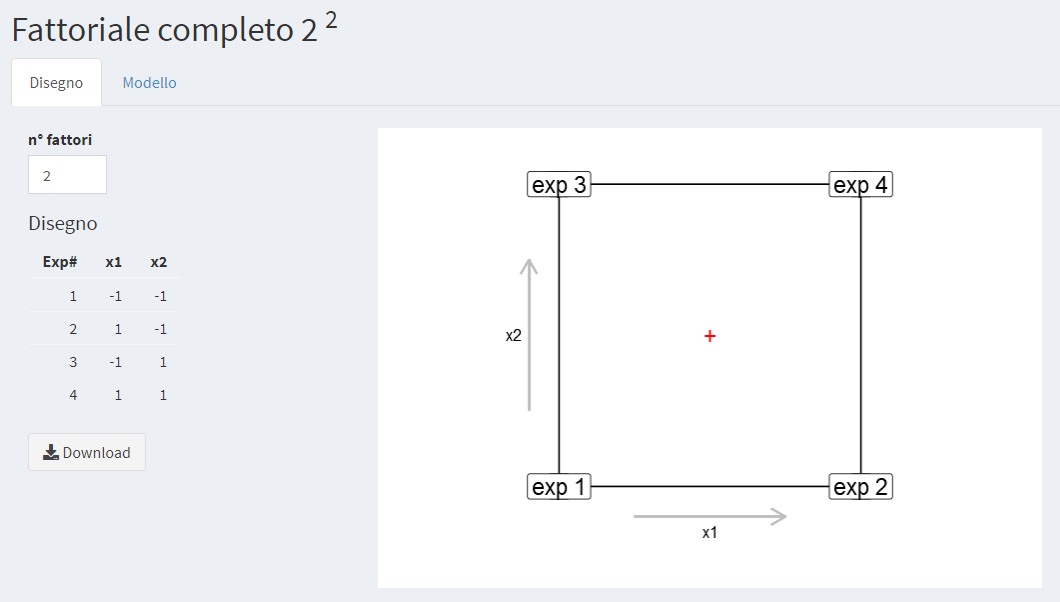
\includegraphics[width=1\linewidth]{Immagini/Fatt_compl/01_fattacompl2liv} 

}

\caption{Disegno fattoriale completo $2^2$}\label{fig:fc1}
\end{figure}

\begin{figure}

{\centering 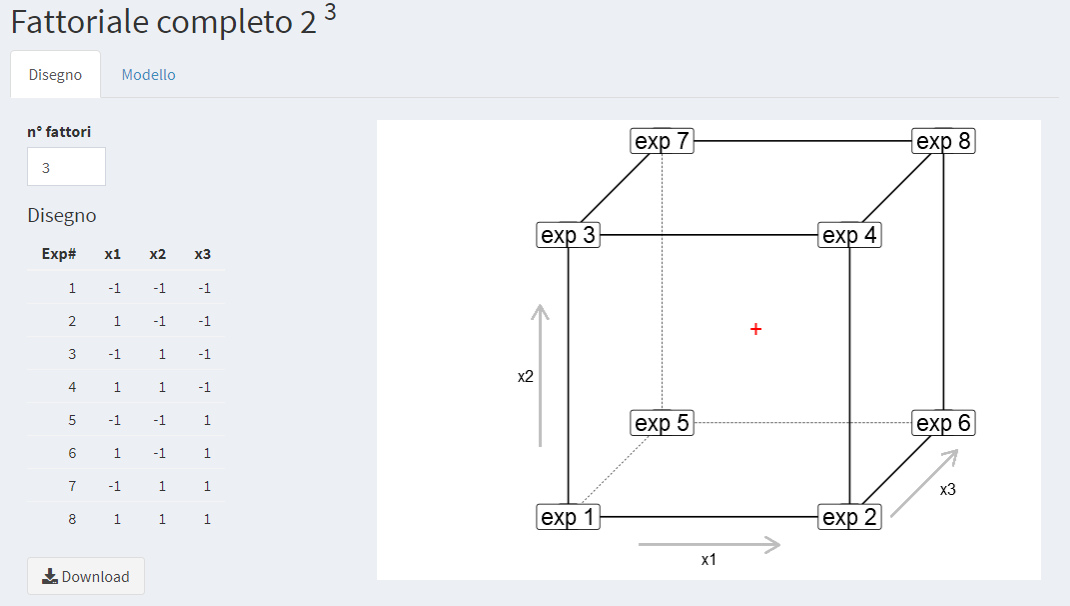
\includegraphics[width=1\linewidth]{Immagini/Fatt_compl/02_fattacompl3liv} 

}

\caption{Disegno fattoriale completo $2^3$}\label{fig:fc2}
\end{figure}

Consideriamo il modello lineare che tiene conto di tutti i termini
lineari e di tutte le possibili interazioni

\begin{equation}
y_i=\beta_0+\beta_1x_{i1}+\cdots+\beta_kx_{ik}+\beta_{12}x_{i1}x_{i2}+\cdots+\beta_{1\dots
k}x_{i1} \cdots x_{ik}+\epsilon_i, \qquad i=1,\dots,2^k, 
\label{eq:ModDisFull}
\end{equation}

dove \(\epsilon_i\sim N(0,\sigma^2)\) a due a due non correlate, errore
sperimentale.\newline La matrice \(X\) del modello è data dalla matrice in Tabella \ref{tab:MatrModDisFull}

\begin{longtable}[]{@{}crrrrrrrc@{}}
\caption{\label{tab:MatrModDisFull} Matrice modello \eqref{eq:ModDisFull}}\tabularnewline
\toprule
\begin{minipage}[b]{0.06\columnwidth}\centering
\strut
\end{minipage} & \begin{minipage}[b]{0.07\columnwidth}\raggedleft
\emph{Int.}\strut
\end{minipage} & \begin{minipage}[b]{0.06\columnwidth}\raggedleft
\(X_1\)\strut
\end{minipage} & \begin{minipage}[b]{0.06\columnwidth}\raggedleft
\(X_2\)\strut
\end{minipage} & \begin{minipage}[b]{0.09\columnwidth}\raggedleft
\(\cdots\)\strut
\end{minipage} & \begin{minipage}[b]{0.06\columnwidth}\raggedleft
\(X_k\)\strut
\end{minipage} & \begin{minipage}[b]{0.09\columnwidth}\raggedleft
\(X_1X_2\)\strut
\end{minipage} & \begin{minipage}[b]{0.09\columnwidth}\raggedleft
\(\cdots\)\strut
\end{minipage} & \begin{minipage}[b]{0.17\columnwidth}\centering
\(X_1X_2\dots X_k\)\strut
\end{minipage}\tabularnewline
\midrule
\endfirsthead
\toprule
\begin{minipage}[b]{0.06\columnwidth}\centering
\strut
\end{minipage} & \begin{minipage}[b]{0.07\columnwidth}\raggedleft
\emph{Int.}\strut
\end{minipage} & \begin{minipage}[b]{0.06\columnwidth}\raggedleft
\(X_1\)\strut
\end{minipage} & \begin{minipage}[b]{0.06\columnwidth}\raggedleft
\(X_2\)\strut
\end{minipage} & \begin{minipage}[b]{0.09\columnwidth}\raggedleft
\(\cdots\)\strut
\end{minipage} & \begin{minipage}[b]{0.06\columnwidth}\raggedleft
\(X_k\)\strut
\end{minipage} & \begin{minipage}[b]{0.09\columnwidth}\raggedleft
\(X_1X_2\)\strut
\end{minipage} & \begin{minipage}[b]{0.09\columnwidth}\raggedleft
\(\cdots\)\strut
\end{minipage} & \begin{minipage}[b]{0.17\columnwidth}\centering
\(X_1X_2\dots X_k\)\strut
\end{minipage}\tabularnewline
\midrule
\endhead
\begin{minipage}[t]{0.06\columnwidth}\centering
1\strut
\end{minipage} & \begin{minipage}[t]{0.07\columnwidth}\raggedleft
1\strut
\end{minipage} & \begin{minipage}[t]{0.06\columnwidth}\raggedleft
-1\strut
\end{minipage} & \begin{minipage}[t]{0.06\columnwidth}\raggedleft
-1\strut
\end{minipage} & \begin{minipage}[t]{0.09\columnwidth}\raggedleft
\(\cdots\)\strut
\end{minipage} & \begin{minipage}[t]{0.06\columnwidth}\raggedleft
-1\strut
\end{minipage} & \begin{minipage}[t]{0.09\columnwidth}\raggedleft
1\strut
\end{minipage} & \begin{minipage}[t]{0.09\columnwidth}\raggedleft
\(\cdots\)\strut
\end{minipage} & \begin{minipage}[t]{0.17\columnwidth}\centering
\((-1)^k\)\strut
\end{minipage}\tabularnewline
\begin{minipage}[t]{0.06\columnwidth}\centering
2\strut
\end{minipage} & \begin{minipage}[t]{0.07\columnwidth}\raggedleft
1\strut
\end{minipage} & \begin{minipage}[t]{0.06\columnwidth}\raggedleft
1\strut
\end{minipage} & \begin{minipage}[t]{0.06\columnwidth}\raggedleft
-1\strut
\end{minipage} & \begin{minipage}[t]{0.09\columnwidth}\raggedleft
\(\cdots\)\strut
\end{minipage} & \begin{minipage}[t]{0.06\columnwidth}\raggedleft
-1\strut
\end{minipage} & \begin{minipage}[t]{0.09\columnwidth}\raggedleft
-1\strut
\end{minipage} & \begin{minipage}[t]{0.09\columnwidth}\raggedleft
\(\cdots\)\strut
\end{minipage} & \begin{minipage}[t]{0.17\columnwidth}\centering
\(\quad (-1)^{k-1}\)\strut
\end{minipage}\tabularnewline
\begin{minipage}[t]{0.06\columnwidth}\centering
3\strut
\end{minipage} & \begin{minipage}[t]{0.07\columnwidth}\raggedleft
1\strut
\end{minipage} & \begin{minipage}[t]{0.06\columnwidth}\raggedleft
-1\strut
\end{minipage} & \begin{minipage}[t]{0.06\columnwidth}\raggedleft
1\strut
\end{minipage} & \begin{minipage}[t]{0.09\columnwidth}\raggedleft
\(\cdots\)\strut
\end{minipage} & \begin{minipage}[t]{0.06\columnwidth}\raggedleft
-1\strut
\end{minipage} & \begin{minipage}[t]{0.09\columnwidth}\raggedleft
-1\strut
\end{minipage} & \begin{minipage}[t]{0.09\columnwidth}\raggedleft
\(\cdots\)\strut
\end{minipage} & \begin{minipage}[t]{0.17\columnwidth}\centering
.\strut
\end{minipage}\tabularnewline
\begin{minipage}[t]{0.06\columnwidth}\centering
4\strut
\end{minipage} & \begin{minipage}[t]{0.07\columnwidth}\raggedleft
1\strut
\end{minipage} & \begin{minipage}[t]{0.06\columnwidth}\raggedleft
1\strut
\end{minipage} & \begin{minipage}[t]{0.06\columnwidth}\raggedleft
1\strut
\end{minipage} & \begin{minipage}[t]{0.09\columnwidth}\raggedleft
\(\cdots\)\strut
\end{minipage} & \begin{minipage}[t]{0.06\columnwidth}\raggedleft
-1\strut
\end{minipage} & \begin{minipage}[t]{0.09\columnwidth}\raggedleft
1\strut
\end{minipage} & \begin{minipage}[t]{0.09\columnwidth}\raggedleft
\(\cdots\)\strut
\end{minipage} & \begin{minipage}[t]{0.17\columnwidth}\centering
.\strut
\end{minipage}\tabularnewline
\begin{minipage}[t]{0.06\columnwidth}\centering
.\strut
\end{minipage} & \begin{minipage}[t]{0.07\columnwidth}\raggedleft
1\strut
\end{minipage} & \begin{minipage}[t]{0.06\columnwidth}\raggedleft
.\strut
\end{minipage} & \begin{minipage}[t]{0.06\columnwidth}\raggedleft
.\strut
\end{minipage} & \begin{minipage}[t]{0.09\columnwidth}\raggedleft
\(\cdots\)\strut
\end{minipage} & \begin{minipage}[t]{0.06\columnwidth}\raggedleft
.\strut
\end{minipage} & \begin{minipage}[t]{0.09\columnwidth}\raggedleft
.\strut
\end{minipage} & \begin{minipage}[t]{0.09\columnwidth}\raggedleft
\(\cdots\)\strut
\end{minipage} & \begin{minipage}[t]{0.17\columnwidth}\centering
.\strut
\end{minipage}\tabularnewline
\begin{minipage}[t]{0.06\columnwidth}\centering
.\strut
\end{minipage} & \begin{minipage}[t]{0.07\columnwidth}\raggedleft
1\strut
\end{minipage} & \begin{minipage}[t]{0.06\columnwidth}\raggedleft
.\strut
\end{minipage} & \begin{minipage}[t]{0.06\columnwidth}\raggedleft
.\strut
\end{minipage} & \begin{minipage}[t]{0.09\columnwidth}\raggedleft
\(\cdots\)\strut
\end{minipage} & \begin{minipage}[t]{0.06\columnwidth}\raggedleft
.\strut
\end{minipage} & \begin{minipage}[t]{0.09\columnwidth}\raggedleft
.\strut
\end{minipage} & \begin{minipage}[t]{0.09\columnwidth}\raggedleft
\(\cdots\)\strut
\end{minipage} & \begin{minipage}[t]{0.17\columnwidth}\centering
.\strut
\end{minipage}\tabularnewline
\begin{minipage}[t]{0.06\columnwidth}\centering
.\strut
\end{minipage} & \begin{minipage}[t]{0.07\columnwidth}\raggedleft
1\strut
\end{minipage} & \begin{minipage}[t]{0.06\columnwidth}\raggedleft
.\strut
\end{minipage} & \begin{minipage}[t]{0.06\columnwidth}\raggedleft
.\strut
\end{minipage} & \begin{minipage}[t]{0.09\columnwidth}\raggedleft
\(\cdots\)\strut
\end{minipage} & \begin{minipage}[t]{0.06\columnwidth}\raggedleft
.\strut
\end{minipage} & \begin{minipage}[t]{0.09\columnwidth}\raggedleft
.\strut
\end{minipage} & \begin{minipage}[t]{0.09\columnwidth}\raggedleft
\(\cdots\)\strut
\end{minipage} & \begin{minipage}[t]{0.17\columnwidth}\centering
.\strut
\end{minipage}\tabularnewline
\begin{minipage}[t]{0.06\columnwidth}\centering
.\strut
\end{minipage} & \begin{minipage}[t]{0.07\columnwidth}\raggedleft
1\strut
\end{minipage} & \begin{minipage}[t]{0.06\columnwidth}\raggedleft
-1\strut
\end{minipage} & \begin{minipage}[t]{0.06\columnwidth}\raggedleft
-1\strut
\end{minipage} & \begin{minipage}[t]{0.09\columnwidth}\raggedleft
\(\cdots\)\strut
\end{minipage} & \begin{minipage}[t]{0.06\columnwidth}\raggedleft
1\strut
\end{minipage} & \begin{minipage}[t]{0.09\columnwidth}\raggedleft
1\strut
\end{minipage} & \begin{minipage}[t]{0.09\columnwidth}\raggedleft
\(\cdots\)\strut
\end{minipage} & \begin{minipage}[t]{0.17\columnwidth}\centering
.\strut
\end{minipage}\tabularnewline
\begin{minipage}[t]{0.06\columnwidth}\centering
.\strut
\end{minipage} & \begin{minipage}[t]{0.07\columnwidth}\raggedleft
1\strut
\end{minipage} & \begin{minipage}[t]{0.06\columnwidth}\raggedleft
1\strut
\end{minipage} & \begin{minipage}[t]{0.06\columnwidth}\raggedleft
-1\strut
\end{minipage} & \begin{minipage}[t]{0.09\columnwidth}\raggedleft
\(\cdots\)\strut
\end{minipage} & \begin{minipage}[t]{0.06\columnwidth}\raggedleft
1\strut
\end{minipage} & \begin{minipage}[t]{0.09\columnwidth}\raggedleft
-1\strut
\end{minipage} & \begin{minipage}[t]{0.09\columnwidth}\raggedleft
\(\cdots\)\strut
\end{minipage} & \begin{minipage}[t]{0.17\columnwidth}\centering
.\strut
\end{minipage}\tabularnewline
\begin{minipage}[t]{0.06\columnwidth}\centering
.\strut
\end{minipage} & \begin{minipage}[t]{0.07\columnwidth}\raggedleft
1\strut
\end{minipage} & \begin{minipage}[t]{0.06\columnwidth}\raggedleft
-1\strut
\end{minipage} & \begin{minipage}[t]{0.06\columnwidth}\raggedleft
1\strut
\end{minipage} & \begin{minipage}[t]{0.09\columnwidth}\raggedleft
\(\cdots\)\strut
\end{minipage} & \begin{minipage}[t]{0.06\columnwidth}\raggedleft
1\strut
\end{minipage} & \begin{minipage}[t]{0.09\columnwidth}\raggedleft
-1\strut
\end{minipage} & \begin{minipage}[t]{0.09\columnwidth}\raggedleft
\(\cdots\)\strut
\end{minipage} & \begin{minipage}[t]{0.17\columnwidth}\centering
.\strut
\end{minipage}\tabularnewline
\begin{minipage}[t]{0.06\columnwidth}\centering
\(2^k\)\strut
\end{minipage} & \begin{minipage}[t]{0.07\columnwidth}\raggedleft
1\strut
\end{minipage} & \begin{minipage}[t]{0.06\columnwidth}\raggedleft
1\strut
\end{minipage} & \begin{minipage}[t]{0.06\columnwidth}\raggedleft
1\strut
\end{minipage} & \begin{minipage}[t]{0.09\columnwidth}\raggedleft
\(\cdots\)\strut
\end{minipage} & \begin{minipage}[t]{0.06\columnwidth}\raggedleft
1\strut
\end{minipage} & \begin{minipage}[t]{0.09\columnwidth}\raggedleft
1\strut
\end{minipage} & \begin{minipage}[t]{0.09\columnwidth}\raggedleft
\(\cdots\)\strut
\end{minipage} & \begin{minipage}[t]{0.17\columnwidth}\centering
1\strut
\end{minipage}\tabularnewline
\bottomrule
\end{longtable}

Poiché la matrice del modello \eqref{eq:ModDisFull} è ortogonale, i
coefficienti relativi ad ogni termine lineare forniscono esattamente
l'informazione di quanto varia la risposta per uno spostamento unitario
del fattore relativo, ossia \(\frac{X_{max}-X_{min}}{2}\), mantenendo gli
altri parametri nulli. E' quindi 1/2 l'\textbf{effetto del parametro},
cioè la differenza tra la media dei valori delle risposte per \(X_{max}\)
e la media dei valori delle risposte per \(X_{min}\).\\
Nell'esempio numerico che trattiamo più avanti, l'effetto del parametro
\(X_1\) (temperatura), vedi Figura \ref{fig:fc5}, è dato dalla differenza
(23) tra la media (75.75) dei 4 valori della faccia \(X_1=1\) e la media
(52.75) dei 4 valori della faccia \(X_1=-1\). Il coefficiente di \(X_1\),
vedi Figura \ref{fig:fc6}, è esattamente 1/2 l'effetto della temperatura.

Più grande in valore assoluto è il coefficiente, e maggiore è l'effetto
del relativo fattore nel dominio sperimentale scelto.

Determinato il vettore \(y\) delle risposte, eseguendo i \(2^k\) esperimenti
nei punti sperimentali individuati dalla matrice sperimentale in
Tabella \ref{tab:MatrDisFull}. (\textbf{Nota importante:} per evitare effetto
di autocorrelazione nell'errore nel modello gli esperimenti non vanno
eseguiti nell'ordine in Tabella \ref{tab:MatrDisFull} ma vanno mischiati
casualmente) dobbiamo stimare

\begin{itemize}
\tightlist
\item
  \(1\) coefficiente interazione \(\beta_0\) (media delle \(2^k\) risposte)
\item
  \(k\) coefficienti termini lineari \(\beta_1,\cdots,\beta_k\)
\item
  in generale \(\frac{k!}{(k-m)!m!}\) coefficienti interazioni di ordine \(m\)
\end{itemize}

Si noti che per il binomio di Newton si ha che
\[
\sum_{m=0}^k\frac{k!}{(k-m)!m!}=2^k. 
\]
La matrice del modello, Tabella \ref{tab:MatrModDisFull}, è quindi un matrice
quadrata \(2^k\)x \(2^k\) e poiché le sue colonne sono a due a due
ortogonali è una matrice di Hadamard.

Dalla teoria della regressione sappiamo che uno stimatore del vettore
dei parametri \(\beta\) del modello \eqref{eq:ModDisFull} è dato dall'unica
soluzione del sistema \(y=Xb\) (si vedano le diapositive \emph{Fattoriale
completo})
\[
 b=X^{-1}y.
\]
e che
\[
Cov(b)=(X^tX)^{-1}=\frac{1}{2^k}I_k
\]
dove con \(I_k\) è indicata la matrice diagonale con valori tutti
uguali a \(1\) sulla diagonale (matrice identità).

Nell'applicativo, scelto il numero di fattori compaiono automaticamente
il modello e la matrice di dispersione (matrice \((X^tX)^{-1}\))
Figura \ref{fig:fc3}

\begin{figure}

{\centering 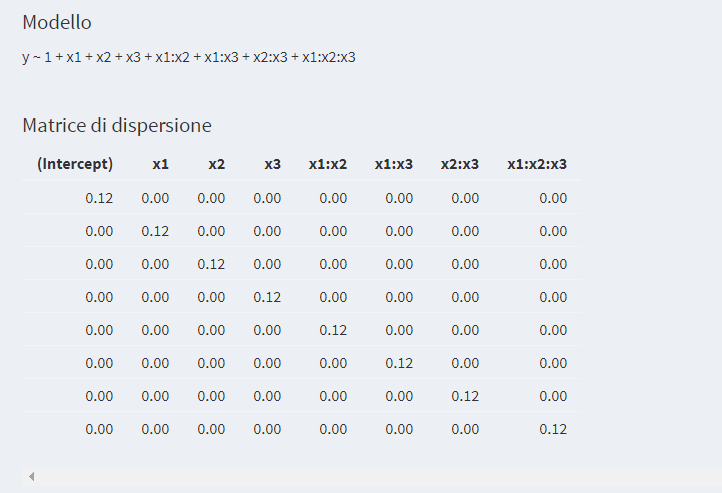
\includegraphics[width=1\linewidth]{Immagini/Fatt_compl/03_matr_disp} 

}

\caption{Modello e matrice di dispersione per un disegno fattoriale completo $2^3$}\label{fig:fc3}
\end{figure}

Come già osservato, la matrice di dispersione è una matrice diagonale, e
questo implica che tutti i fattori sono ortogonali tra di loro
\[
Corr(b_i,b_j)=0, \qquad i\neq j
\]
Il coefficiente \(\beta_j\) non cambia anche se elimino qualche
fattore, o anche tutti i fattori \(X_i,\) \(i\neq j\) dal modello (la
variazione dovuta da \(X_j\) sulla risposta è letta soltanto da
\(\beta_j\)).

Inoltre per lo stimatore \(b=X^{-1}y\) abbiamo che

\begin{equation}
Var(b_j)=\frac{\sigma^2}{2^k},
\qquad j=1,\dots,2^k 
\label{eq:VarFull}
\end{equation}

La \eqref{eq:VarFull} ci dice la qualità dell'informazione dello
stimatore \(b_j\). Ci permette inoltre di studiare la significatività
statistica di \(\beta_j\) nota la varianza sperimentale \(\sigma^2\).

Essendo \(y=Xb\) un sistema di \(2^k\) equazioni (linearmente indipendenti)
in \(2^k\) incognite, non abbiamo gradi di libertà, e quindi non siamo in
grado di stimare \(\sigma^2\). Alla fine di questo paragrafo vedremo, se
non è nota a priori la varianza \(\sigma^2\), come possiamo superare
questo ostacolo.

Il valore previsto dal modello in un punto \((x_1,x_2,\dots,x_k)\) del
dominio sperimentale è dato da
\[
\hat{y_0}=x_0b
\]
dove \(x_0=(1,x_1,\dots,x_1x_2,\dots,x_1x_2\cdots x_k)\) (riga della
matrice del modello Tabella \ref{tab:MatrDisFull} corrispondente al punto
\((x_1,x_2,\dots,x_k)\)). Dalla teoria sappiamo che la varianza dello
stimatore \(\hat{y_0}\) è data da
\[
Var(\hat{y_0})=x_0(X^tX)^{-1}x_0^t\sigma^2
\]
La quantità \(x_0(X^tX)^{-1}x_0^t\) è chiamata \emph{Leverage} nel punto
\((x_1,x_2,\dots,x_k)\).

Nell'applicativo si trova il grafico del leverage per ogni punto del
dominio, Figura \ref{fig:fc4}

\begin{figure}

{\centering 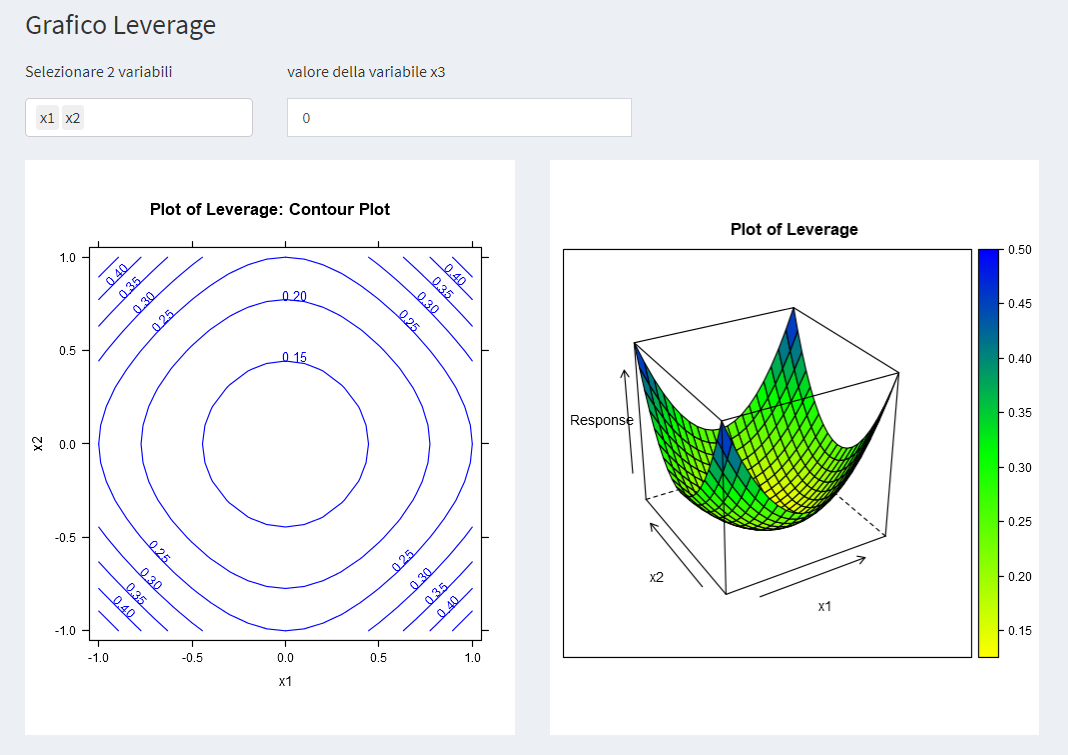
\includegraphics[width=1\linewidth]{Immagini/Fatt_compl/04_lev} 

}

\caption{Linee di livello e superficie del leverage per un disegno fattoriale completo $2^3$}\label{fig:fc4}
\end{figure}

La superficie di leverege ci dice com'è la qualità dell'informazione
dello stimatore risposta in ogni punto del dominio sperimentale.

A questo punto è opportuno fare due osservazioni importanti:

\begin{enumerate}
\def\labelenumi{\arabic{enumi})}
\item
  il leverage non dipende dai valori delle risposte. Per questo si
  trova nel sotto-menù \emph{Disegno} il cui output dipende solo dal
  disegno.
\item
  nei punti del disegno, poiché la somma dei quadrati dei valori delle
  righe della matrice del modello Tabella \ref{tab:MatrDisFull}è \(2^k\), il
  valore del leverage è \(1\).\\
  Questo significa che il modello ``deve passare'' per quei punti, ma
  questo non deve meravigliare poiché, coma già detto, non abbiamo
  gradi di libertà. Per fissare le idee su questo passaggio
  fondamentale, siamo nello stessa situazione che conosciamo nel piano
  quando abbiamo solo due punti per stimare i coefficienti di una
  retta.
\end{enumerate}

Si noti che i \(2^k\) punti sperimentali sono i punti del dominio
sperimentale di leverage massimo. Il che significa che in ognuno di
questi punti l'informazione che abbiamo grazie al modello è migliore di
quella che avremmo mediante un (unico) eventuale esperimento in quel
punto. Ciò significa che la risposta, o meglio l'aspettativa della
risposta, può essere predetta meglio (leggi con varianza minore) dal
modello che da un singolo esperimento in quel punto. \newline

Consideriamo ora un esempio numerico.\\
Supponiamo ora di dover identificare le condizioni di processo di una
reazione chimica. Vogliamo determinare l'influenza di 3 fattori

\begin{itemize}
\item
  \(X_1\): temperatura (°C)
\item
  \(X_2\): concentrazione del substrato (\%, p/p)
\item
  \(X_3\): tipo di catalizzatore
\end{itemize}

e delle loro interazioni sulla risposta

\begin{itemize}
\tightlist
\item
  \(Y\): resa di reazione
\end{itemize}

Dobbiamo innanzitutto scegliere il dominio sperimentale, cioè per ogni
fattore dobbiamo determinare un intervallo di valori compreso tra un
massimo e un minimo entro i quali studiare il fenomeno a cui siamo
interessati. Abbiamo 2 fattori quantitativi, che sono la temperatura e
la concentrazione del substrato, e un fattore qualitativo a 2 livelli, e
questo è il tipo di catalizzatore: A o B.

\begin{longtable}[]{@{}lrr@{}}
\caption{\label{tab:livelli}Definizione dei livelli}\tabularnewline
\toprule
Fattori & -1 & +1\tabularnewline
\midrule
\endfirsthead
\toprule
Fattori & -1 & +1\tabularnewline
\midrule
\endhead
temperatura & 160 & 180\tabularnewline
concentrazione & 20 & 40\tabularnewline
catalizzatore & A & B\tabularnewline
\bottomrule
\end{longtable}

La matrice del disegno Tabella \ref{tab:MatrDisFull} per 3 fattori è quella in Figura \ref{fig:fc2}. Il piano degli esperimenti Tabella \ref{tab:esperimenti} si
ottiene sostituendo a -1/+1 il valore corrispondente nella Tabella
\ref{tab:livelli}. \newpage

\begin{longtable}[]{@{}cccc@{}}
\caption{\label{tab:esperimenti}Piano degli esperimenti}\tabularnewline
\toprule
Exp. & Temp & Conc & Cat\tabularnewline
\midrule
\endfirsthead
\toprule
Exp. & Temp & Conc & Cat\tabularnewline
\midrule
\endhead
1 & 160 & 20 & A\tabularnewline
2 & 180 & 20 & A\tabularnewline
3 & 160 & 40 & A\tabularnewline
4 & 180 & 40 & A\tabularnewline
5 & 160 & 20 & B\tabularnewline
6 & 180 & 20 & B\tabularnewline
7 & 160 & 40 & B\tabularnewline
8 & 180 & 40 & B\tabularnewline
\bottomrule
\end{longtable}

Gli esperimenti sono elencati nel cosiddetto ``ordine standard''. Per
evitare di osservare effetti (errori) sistematici, gli esperimenti
devono essere eseguiti in ordine casuale (random order). Alla fine degli
esperimenti otteniamo i risultati in Tabella \ref{tab:esperimentir}

\begin{longtable}[]{@{}ccccc@{}}
\caption{\label{tab:esperimentir}Piano degli esperimenti con risposte}\tabularnewline
\toprule
Exp. & Temp & Conc & Cat & Resa\tabularnewline
\midrule
\endfirsthead
\toprule
Exp. & Temp & Conc & Cat & Resa\tabularnewline
\midrule
\endhead
1 & 160 & 20 & A & 60\tabularnewline
2 & 180 & 20 & A & 72\tabularnewline
3 & 160 & 40 & A & 54\tabularnewline
4 & 180 & 40 & A & 68\tabularnewline
5 & 160 & 20 & B & 52\tabularnewline
6 & 180 & 20 & B & 83\tabularnewline
7 & 160 & 40 & B & 45\tabularnewline
8 & 180 & 40 & B & 80\tabularnewline
\bottomrule
\end{longtable}

Per inserire le risposte nell'applicativo bisogna andare nel sotto menu
\emph{Modello} e inserire le risposte nell'apposito riquadro, vedi Figura
\ref{fig:fc5} (da Excel basta copiare la colonna delle risposte e
incollarla nel riquadro)

\begin{figure}

{\centering 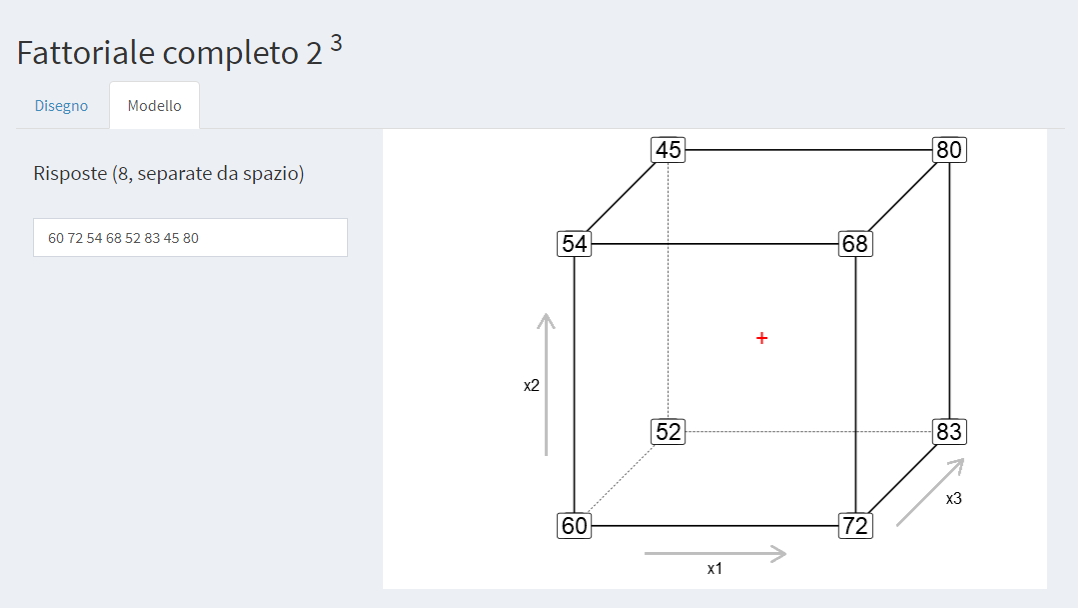
\includegraphics[width=1\linewidth]{Immagini/Fatt_compl/05_risp} 

}

\caption{Inserimento risposte nell'applicativo}\label{fig:fc5}
\end{figure}

Per un numero di fattori non superiore a 3 viene fornita anche una
rappresentazione grafica delle risposte.

Una volta inserite le risposte, il calcolo dei coefficienti del modello
è automatico e ne abbiamo anche una rappresentazione grafica, vedi
Figura \ref{fig:fc6}

\begin{figure}

{\centering 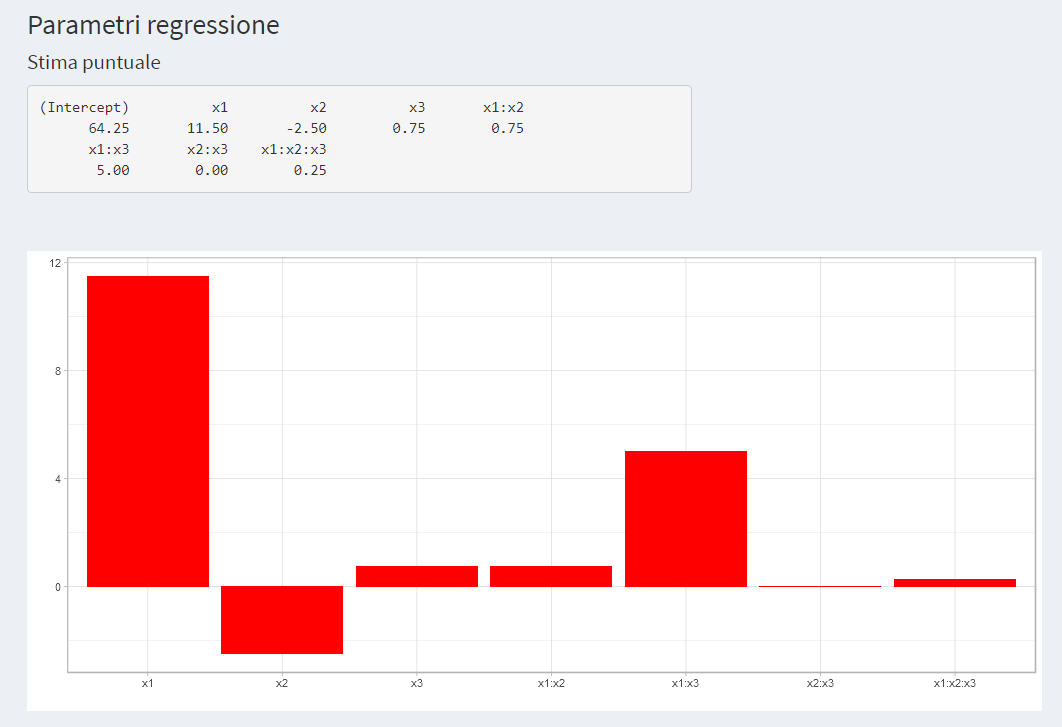
\includegraphics[width=1\linewidth]{Immagini/Fatt_compl/06_coeff} 

}

\caption{Calcolo dei coefficienti del modello}\label{fig:fc6}
\end{figure}

Un altro grafico riportato è il \emph{Grafico degli effetti normalizzati},
Figura \ref{fig:fc7}, in cui sono rappresentati i coefficienti che
contribuiscono di più nel determinare la risposta. Il grafico
rappresenta la percentuale del contributo di ciascun coefficiente
elevato al quadrato alla somma dei quadrati di tutti i coefficienti. I
coefficienti che risultano dare un contributo in percentuale maggiore
sono quelli che che influenzano maggiormente la risposta.

\begin{figure}

{\centering 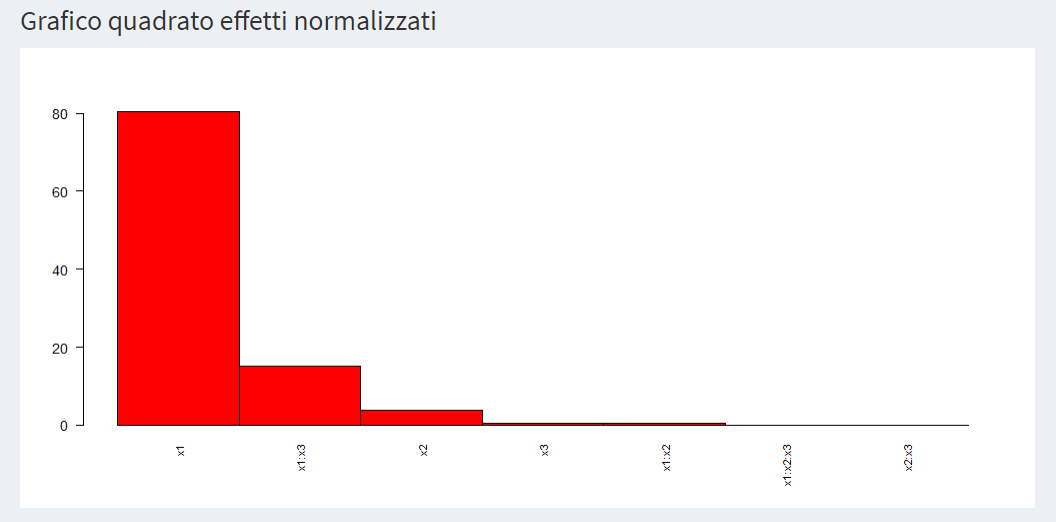
\includegraphics[width=1\linewidth]{Immagini/Fatt_compl/07_coeff_norm} 

}

\caption{Grafico degli effetti normalizzati}\label{fig:fc7}
\end{figure}

Dai grafici Figura \ref{fig:fc6} e Figura \ref{fig:fc7} risulta che i fattori
che influenzano di più la risposta Resa sono la temperatura e la sua
interazione con il tipo di catalizzatore.\\
In Figura \ref{fig:fc8} è illustrato il grafico della superficie di
risposta della Resa in funzione della temperatura e del tipo di
catalizzatore, avendo fissato la concentrazione del substrato nel punto
centrale del suo intervallo di variazione, vale a dire al 30\%.

\begin{figure}

{\centering 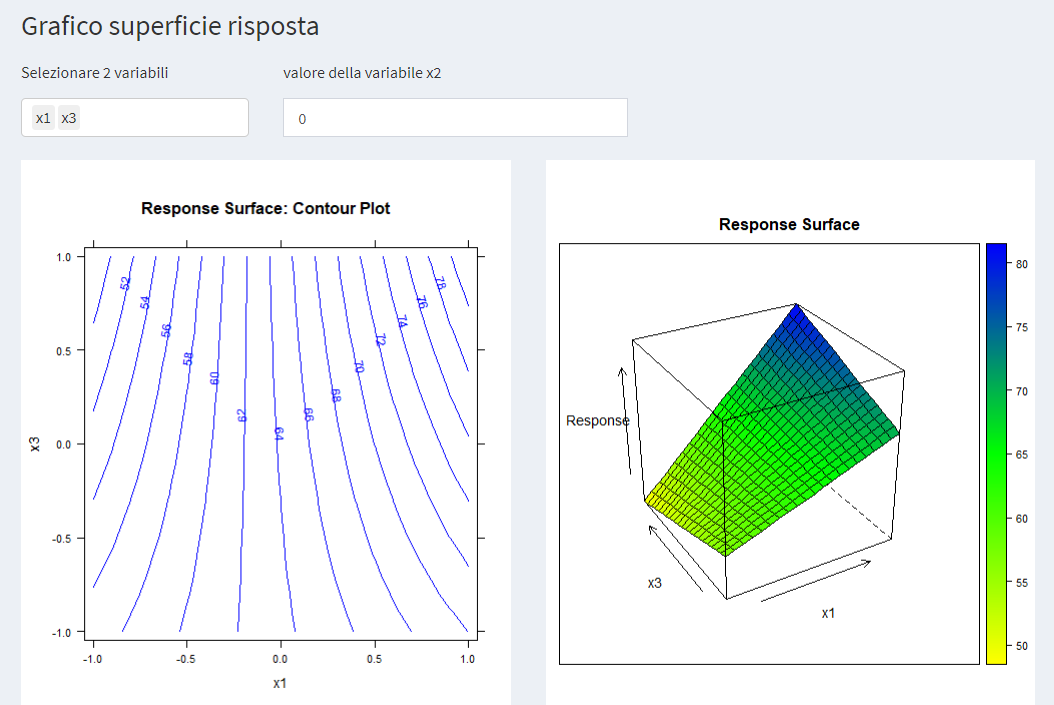
\includegraphics[width=1\linewidth]{Immagini/Fatt_compl/08_sup_risp} 

}

\caption{Grafico della superficie di risposta della Resa}\label{fig:fc8}
\end{figure}

Come si nota dalla Figura \ref{fig:fc8} il massimo della resa si ottiene
alla temperatura massima (180 °C) e usando il catalizzatore del tipo B
quando il substrato è alla concentrazione del 30\%.

Circa la significatività dei coefficienti, per quanto già osservato
precedentemente, non abbiamo gradi di libertà e quindi non è possibile
stimare \(\sigma^2\).

Una analisi grafica della significatività dei parametri \(b_j\) può essere
effettuata mediante il \emph{Normal Probability Plot}, Figura \ref{fig:fc9}. Se
tutti i coefficienti fossero nulli, i.e.~se fossero tutti distribuiti
come una normale di media \(0\) e varianza \(\sigma^2/2^k\), essi sarebbero
distribuiti come una retta. Possiamo considerare significativamente non
nulli i coefficienti che si discostano dalla retta.

\begin{figure}

{\centering 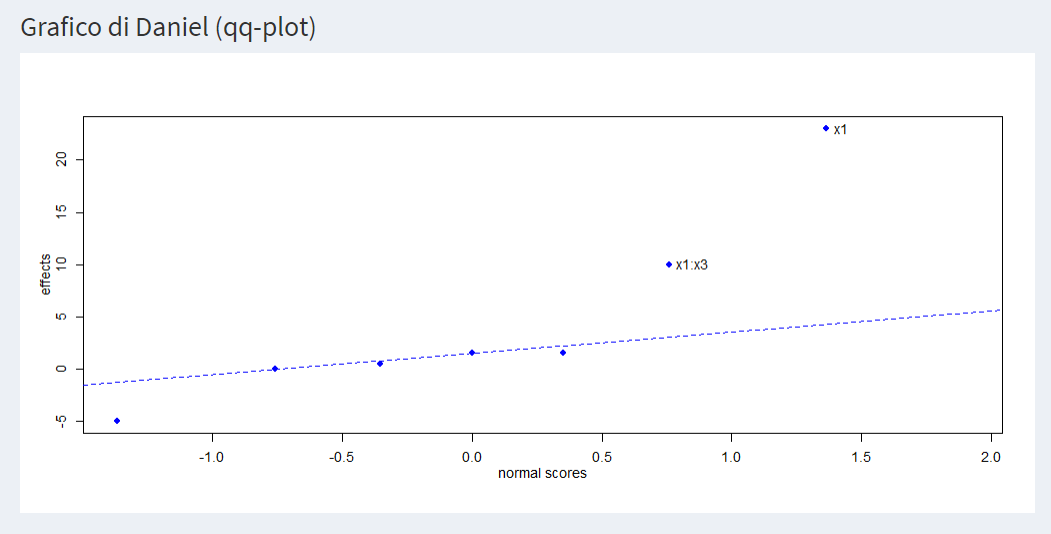
\includegraphics[width=1\linewidth]{Immagini/Fatt_compl/09_qqplot} 

}

\caption{qq-plot dei coefficienti}\label{fig:fc9}
\end{figure}

Dal qq-plot in Figura \ref{fig:fc9} si ottiene la conferma che sono
significativi (leggi: diversi da zero) la temperatura e la sua
interazione con il tipo di catalizzatore.

Per convalidare il modello eseguiamo alcune misure indipendenti
\(\eta_1,\dots,\eta_p\) in un punto del dominio scelto arbitrariamente. In
generale si prende il centro del dominio perché è il punto in cui il
leverage è minore. Possiamo determinare \(\sigma^2\) con lo stimatore \[
s^2=\frac{1}{p-1}\sum_{p=1}^p(\eta_i-\bar{\eta})^2.
\] Possiamo costruire l'intervallo di confidenza della misura ``vera'' in
quel punto \[
\bar{\eta}\pm t(\alpha/2,p-1)s\sqrt{1/p}
\] per \(\alpha\) fissato (in generale \(\alpha=95\%\)).

Nel nostro caso essendo il terzo fattore qualitativo prendiamo il punto
centrale tra la temperatura e la concentrazione per il catalizzatore di
tipo B, ossia il punto \((X_1,X_2,X_3)=(0,0,1)\).\\
Inserendo il valore delle misure indipendenti nell'applicativo,
Figura \ref{fig:fc10} otteniamo il valore medio delle misure e il relativo
intervallo di confidenza al 95\%, quindi il valore della deviazione
standard e dei gradi di libertà.

\begin{figure}

{\centering 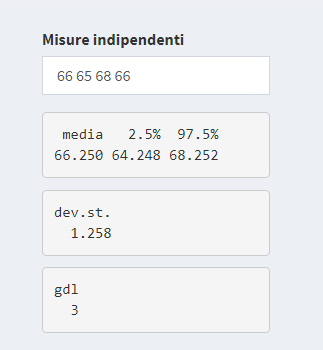
\includegraphics[width=1\linewidth]{Immagini/Fatt_compl/10_mis_ind} 

}

\caption{Misure indipendenti}\label{fig:fc10}
\end{figure}

Inserendo le misure indipendenti abbiamo quindi una stima di \(\sigma\) e
dei gradi di libertà. Utilizzando questi valori è possibile, grazie
all'equazione \eqref{eq:VarFull}, costruire l'intervallo di confidenza dei
parametri del modello. Nell'applicativo si ottengono gli estremi degli
intervalli di confidenza dei parametri per alcuni valori di \(\alpha\) e i
relativi \(p-value\), Figura \ref{fig:fc11}

\begin{figure}

{\centering 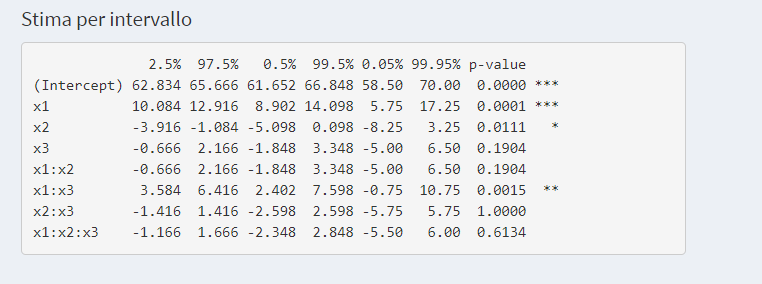
\includegraphics[width=1\linewidth]{Immagini/Fatt_compl/11_intconf} 

}

\caption{Estremi degli intervalli di confidenza dei coefficienti}\label{fig:fc11}
\end{figure}

Nel grafico dei parametri, l'ampiezza degli intervalli di confidenza è
rapprentata con un segmento di colore verde, Figura \ref{fig:fc12}

\begin{figure}

{\centering 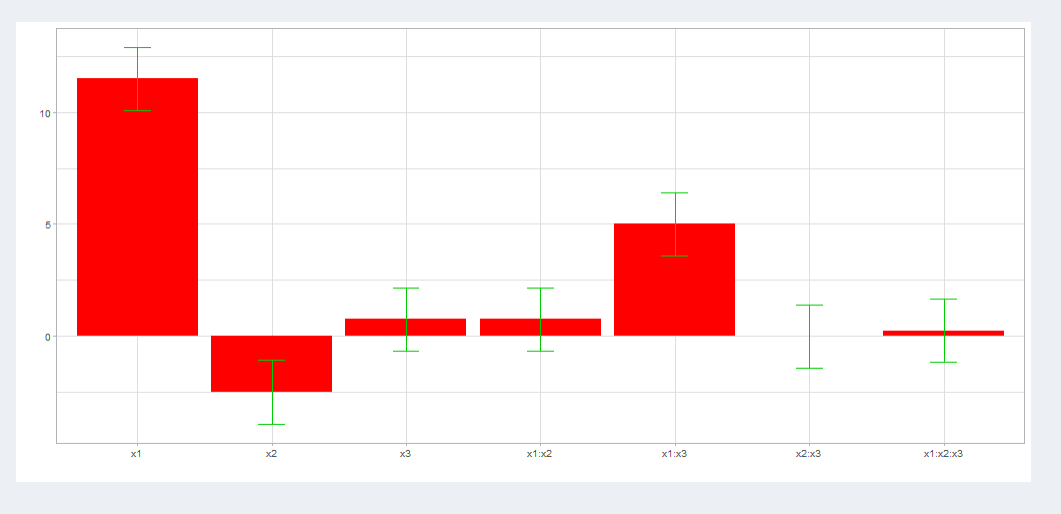
\includegraphics[width=1\linewidth]{Immagini/Fatt_compl/12_intcong_graf} 

}

\caption{Grafico dei coefficienti con estrremi degli intervalli di confidenza dei coefficienti}\label{fig:fc12}
\end{figure}

Per convalidare il modello bisogna quindi vedere quale è il valore
previsto dal modello nel punto in cui abbiamo eseguito le misure
indipendenti e verificare che non differisca significativamente dal
valore ottenuto dalle misure indipendenti (ossia appartenga
all'intervallo di confidenza determinato).\\
Inserendo nell'applicativo le coordinate del punto in cui sono state
eseguite le misure indipendenti otteniamo la previsione del modello in
quel punto e gli estremi dell'intervallo di confidenza costruiti con la
stima di \(\sigma\) ottenuta, Figura \ref{fig:fc13}

\begin{figure}

{\centering 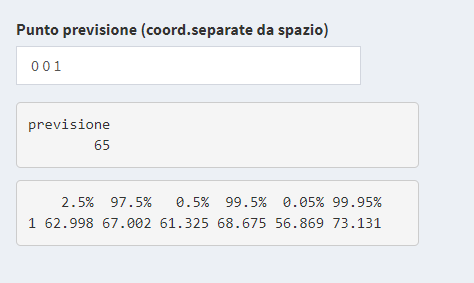
\includegraphics[width=1\linewidth]{Immagini/Fatt_compl/13_prev} 

}

\caption{Previsione del modello in un punto}\label{fig:fc13}
\end{figure}

Nel nostro esempio numerico il modello risulta convalidato.

\hypertarget{disegni-frazionari}{%
\chapter{Disegni Frazionari}\label{disegni-frazionari}}

All'aumentare del numero \(k\) dei fattori, il numero degli esperimenti da eseguire in un disegno fattoriale completo (a 2 livelli) aumenta esponenzialmente come \(2^k\).\\
In Tabella \ref{tab:exprich} è riportato il numero di esperimenti richiesti in funzione del numero di fattori \(k\) nei piani sperimentali fattoriali completi.

\begin{table}

\caption{\label{tab:exprich}Esperimenti richiesti per disegni fattoriali completi $2^k$}
\centering
\begin{tabular}[t]{cc}
\toprule
Fattori (k) & Esperimenti (2\textasciicircum{}k)\\
\midrule
4 & 16\\
5 & 32\\
6 & 64\\
7 & 128\\
8 & 256\\
\addlinespace
9 & 512\\
\bottomrule
\end{tabular}
\end{table}

E' possibile ridurre il numero di esperimenti, riducendolo di \(\frac{1}{2},\frac{1}{4}, \dots\), costruendo a partire da un disegno fattoriale completo \(2^k\) un disegno fattoriale frazionario \(2^{k-p}\) pur di accettare di ``confondere'' tra loro alcuni termini del modello. In generale, la strategia per fare questo consiste nel cercare di ``confondere'' termini di ordine maggiore che possono essere considerati trascurabili a priori, secondo il principio empirico della economia degli effetti (v. \protect\hyperlink{glossario}{Glossario}).

Vediamo come possiamo costruire un disegno frazionario \(2^{k-p}\) con un esempio specifico.\\
Supponiamo di voler costruire il disegno \(2^{5-2}\) ossia \(1/4\) del disegno fattoriale completo \(2^5\).\\
Partiamo dal disegno \(2^3\), vedi Tabella \ref{tab:fatt3}

\begin{table}

\caption{\label{tab:fatt3}Disegno fattorialo completo $2^3$}
\centering
\begin{tabular}[t]{rrr}
\toprule
x1 & x2 & x3\\
\midrule
-1 & -1 & -1\\
1 & -1 & -1\\
-1 & 1 & -1\\
1 & 1 & -1\\
-1 & -1 & 1\\
\addlinespace
1 & -1 & 1\\
-1 & 1 & 1\\
1 & 1 & 1\\
\bottomrule
\end{tabular}
\end{table}

a cui dobbiamo aggiungere i fattori mancanti \(x_4\) e \(x_5\) ``confondendoli'' con le interazioni \(x_4=x_1x_2\) e \(x_5=x_1x_3\). Otteniamo così il disegno Tabella \ref{tab:fraz52} in cui la quarta colonna risulta il prodotto della prima con seconda e la quinta il prodotto tra la prima e la terza \newpage

\begin{table}

\caption{\label{tab:fraz52}Disegno frazionario $2^{5-2}$}
\centering
\begin{tabular}[t]{rrrrr}
\toprule
x1 & x2 & x3 & x4 & x5\\
\midrule
-1 & -1 & -1 & 1 & 1\\
1 & -1 & -1 & -1 & -1\\
-1 & 1 & -1 & -1 & 1\\
1 & 1 & -1 & 1 & -1\\
-1 & -1 & 1 & 1 & -1\\
\addlinespace
1 & -1 & 1 & -1 & 1\\
-1 & 1 & 1 & -1 & -1\\
1 & 1 & 1 & 1 & 1\\
\bottomrule
\end{tabular}
\end{table}

Diremo che \(x_4=x_1x_2\) e \(x_5=x_1x_3\) sono i generatori del disegno frazionario \(2^{5-2}\).

Nell'applicativo, nel menù \emph{Frazionario}, vengono costruiti i disegni frazionari \(2^{k-p}\) indicando il numero di fattori \(k\) e il numero di generatori \(p\).\\
In Figura \ref{fig:fz1} abbiamo il risultato che si ottiene per \(k=5\) e \(p=2\), ossia il disegno \(2^{5-2}\).

\begin{figure}[ht]

{\centering 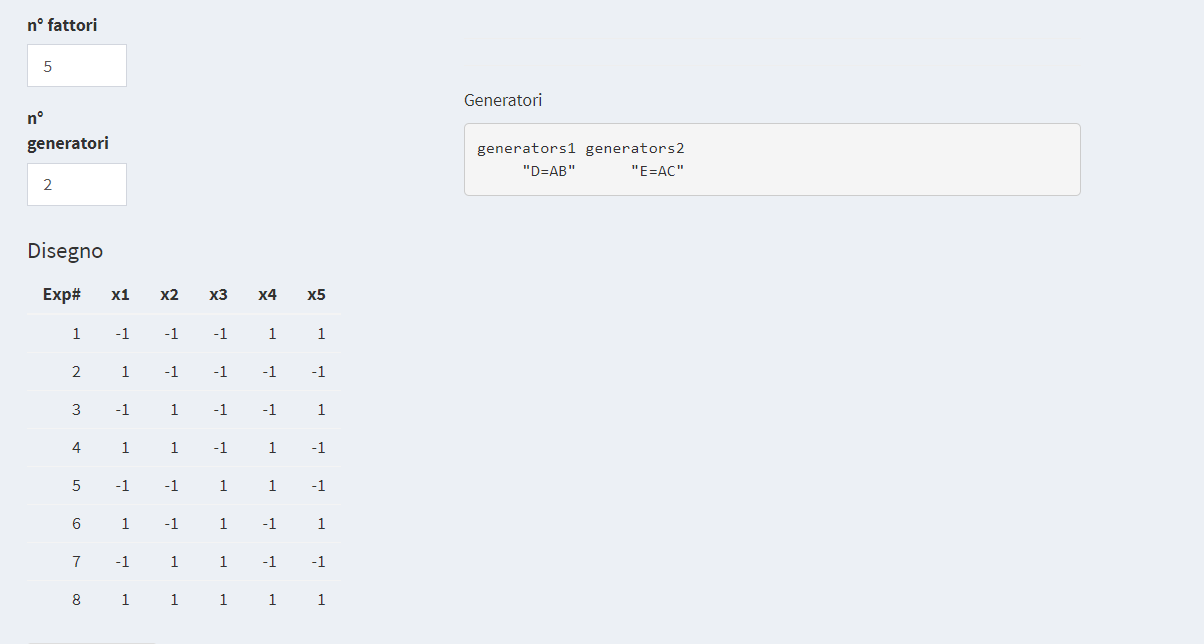
\includegraphics[width=1\linewidth]{Immagini/Fraz/01_fraz} 

}

\caption{Disegno frazionario $2^{5-2}$}\label{fig:fz1}
\end{figure}

Si noti che i generatori sono indicati con le lettere maiuscole, e che queste corrispondono alle colonne della matrice disposte in ordine alfabetico (A è la prima colonna, B la seconda, C la terza, D la quarta ed E la quinta colonna)

Poiché ogni colonna della matrice del disegno elevata al quadrato è la colonna cosiddetta \emph{identità}, \emph{Int.}, costituita solo da valori uguali a 1, dalle relazioni \(x_4=x_1x_2\) e \(x_5=x_1x_3\) si ottiene facilmente che
\[
Int.=x_1x_2x_4 \qquad \rm{e} \qquad \it{Int.}=x_1x_3x_5
\]
dette \emph{Relazioni di identità}. La lunghezza (ordine delle interazioni) minima delle relazioni d'identità è chiamata \emph{risoluzione} del disegno e, di solito, è indicata con un numero romano. Nel nostro esempio la risoluzione è \(III\) e il disegno viene indicato con \(2^{5-2}_{III}\).\\
In linea di principio conviene scegliere relazioni di risoluzione massima (V e superiore) in quanto confondono termini di ordine maggiore. Questa di solito è l'indicazione data dalla maggior parte dei software professionali commerciali (v. Figura \ref{fig:fz2}). Ma affinando l'esperienza e la pratica nell'uso dei fattoriali frazionari si constateranno le notevoli potenzialità offerte anche da disegni di ordine III e IV.

Nella Figura \ref{fig:fz2}, è riportata la copia della prima schermata da Design Expert®: sono indicati i disegni frazionari che si possono costruire in funzione del numero di fattori (per colonna) e numero di esperimenti (per riga) con la relativa risoluzione.

\begin{figure}[ht]

{\centering 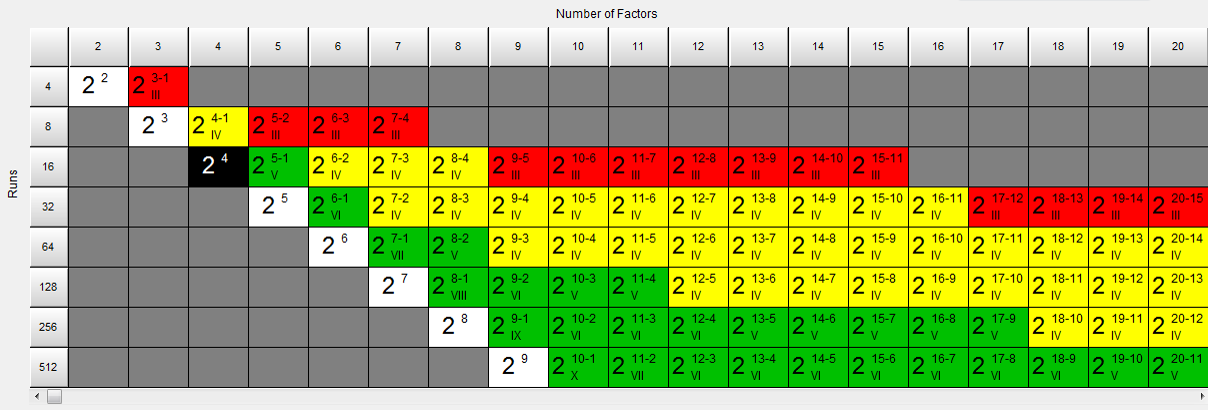
\includegraphics[width=1\linewidth]{Immagini/Fraz/02_risoluzione} 

}

\caption{Disegni frazionari con risoluzione}\label{fig:fz2}
\end{figure}

Per la ragione detta sopra, i programmatori di Design Expert® hanno assegnato dei codici-colore ``semaforici'' ai diversi disegni frazionari. Il colore del riquadro corrisponde al rischio di ottenere risultati inconcludenti. Perciò disegni con risoluzione \(III\), in cui si ``confondono'' i termini lineari con le interazioni di ordine 2 sono colorati in rosso (rischio/attenzione alti); i disegni di risoluzione \(IV\) in cui si ``confondono'' i termini lineari con le interazioni di ordine 3, e le interazioni di ordine 2 sono confuse a coppie tra loro, sono in giallo (rischio/attenzione medi). In verde, invece, sono indicati i disegni di risoluzione superiore a V (via libera, nessuna attenzione?). Questo tipo di classificazione è discutibile, come detto, ed è da considerare al pari di un consiglio di prudenza, peraltro scontato, perché l'uso dei fattoriali frazionari è da pensare per risolvere il problema chimico in esame, e non viceversa (i.e.~come adattare il problema ad un disegno frazionario di risoluzione sufficientemente alta).
La Figura \ref{fig:fz2} è la prima immagine del menù \emph{Frazionari} dell'applicativo.

Con semplice algebra, sempre osservando che \(x_i^2=Int.\), i.e.~ogni colonna al quadrato è la colonna identità \(Int.\) formata da tutti 1, si ottengono tutte le altre ``confusioni''.\\
Nell'applicativo compaiono automaticamente sia il modello relativo al disegno sia tutte le ``confusioni'', vedi Figura \ref{fig:fz3}

\begin{figure}[ht]

{\centering 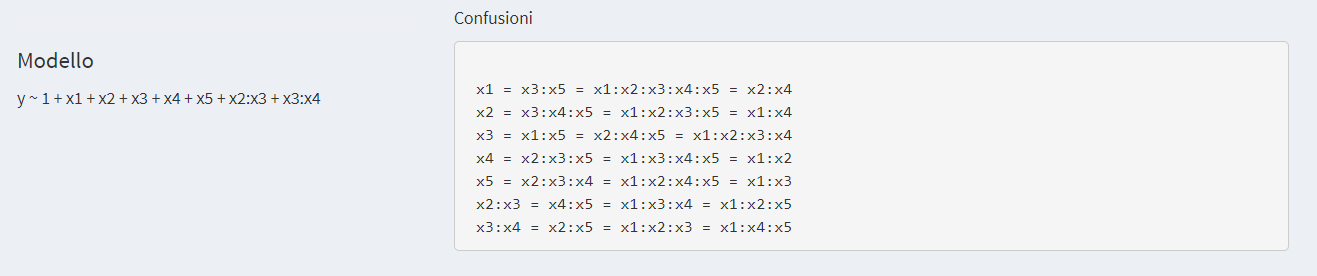
\includegraphics[width=1\linewidth]{Immagini/Fraz/03_confusioni} 

}

\caption{Modello e confusioni del disegno frazionario $2_{III}^{5-2}$}\label{fig:fz3}
\end{figure}

Per quanto riguarda la rimanente parte di output, tutto è presentato nella stessa logica già vista per i disegni fattoriali completi.

\hypertarget{esempio-confusioni}{%
\section{Esempio: confusioni}\label{esempio-confusioni}}

Per comprendere meglio le ``confusioni'' in un disegno frazionario consideriamo il seguente esempio didattico. Supponiamo che il modello ``vero'' (quello che a priori non conosciamo) del fenomeno di studio sia il seguente
\[
y=x_1+5x_2-3x_3+15x_1x_3+\epsilon
\]
Nella progettazione degli esperimenti per studiare il fenomeno in osservazione abbiamo ipotizzato che la risposta dipenda da 5 fattori \(x_1,x_2,x_3,x_4,x_5\).

Per studiare tutte le possibili interazioni consideriamo un disegno fattoriale completo Tabella \ref{tab:Conffull}

\begin{table}

\caption{\label{tab:Conffull}Disegno fattoriale completo $2^5$ (32 esperimenti) con risposte costruito dal modello "vero" ipotizzato $y=x_1+5x_2-3x_3+15x_1x_3+\epsilon$}
\centering
\begin{tabular}[t]{rrrrrr}
\toprule
x1 & x2 & x3 & x4 & x5 & y\\
\midrule
-1 & -1 & -1 & -1 & -1 & 11.96\\
1 & -1 & -1 & -1 & -1 & -17.15\\
-1 & 1 & -1 & -1 & -1 & 23.23\\
1 & 1 & -1 & -1 & -1 & -5.04\\
-1 & -1 & 1 & -1 & -1 & -22.91\\
\addlinespace
1 & -1 & 1 & -1 & -1 & 5.90\\
-1 & 1 & 1 & -1 & -1 & -12.81\\
1 & 1 & 1 & -1 & -1 & 18.18\\
-1 & -1 & -1 & 1 & -1 & 11.56\\
1 & -1 & -1 & 1 & -1 & -17.82\\
\addlinespace
-1 & 1 & -1 & 1 & -1 & 20.86\\
1 & 1 & -1 & 1 & -1 & -6.44\\
-1 & -1 & 1 & 1 & -1 & -24.14\\
1 & -1 & 1 & 1 & -1 & 9.41\\
-1 & 1 & 1 & 1 & -1 & -13.74\\
\addlinespace
1 & 1 & 1 & 1 & -1 & 16.17\\
-1 & -1 & -1 & -1 & 1 & 11.64\\
1 & -1 & -1 & -1 & 1 & -14.71\\
-1 & 1 & -1 & -1 & 1 & 20.62\\
1 & 1 & -1 & -1 & 1 & -5.95\\
\addlinespace
-1 & -1 & 1 & -1 & 1 & -23.92\\
1 & -1 & 1 & -1 & 1 & 7.07\\
-1 & 1 & 1 & -1 & 1 & -13.31\\
1 & 1 & 1 & -1 & 1 & 17.66\\
-1 & -1 & -1 & 1 & 1 & 11.69\\
\addlinespace
1 & -1 & -1 & 1 & 1 & -15.81\\
-1 & 1 & -1 & 1 & 1 & 21.73\\
1 & 1 & -1 & 1 & 1 & -4.59\\
-1 & -1 & 1 & 1 & 1 & -24.53\\
1 & -1 & 1 & 1 & 1 & 6.81\\
\addlinespace
-1 & 1 & 1 & 1 & 1 & -13.02\\
1 & 1 & 1 & 1 & 1 & 18.17\\
\bottomrule
\end{tabular}
\end{table}

Il cui grafico dei coefficienti è dato in Figura \ref{fig:fz11}.

\begin{figure}[ht]

{\centering 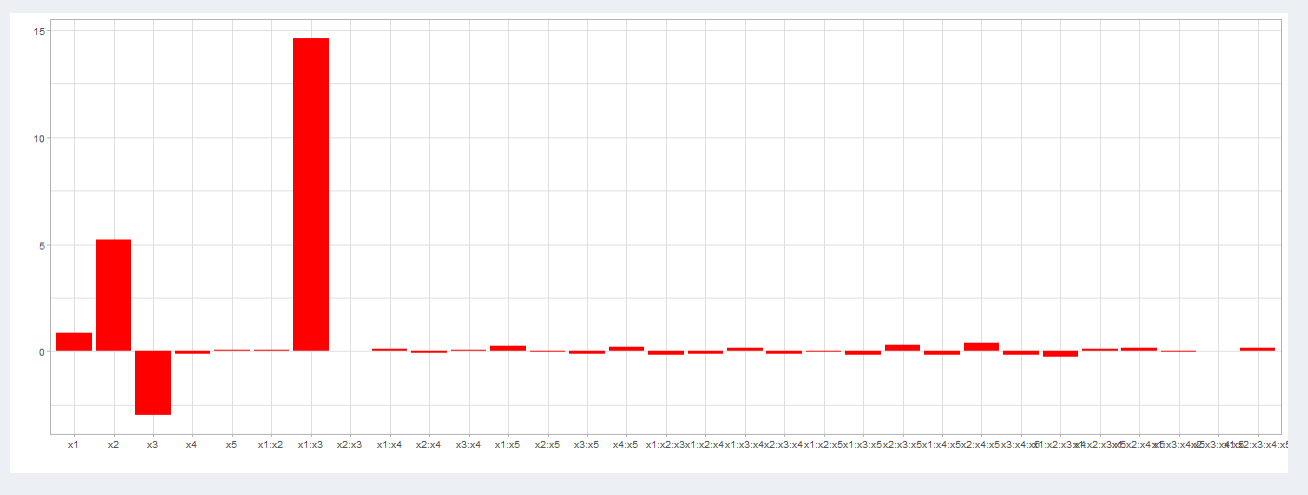
\includegraphics[width=1\linewidth]{Immagini/Fraz/11_Conf_full2} 

}

\caption{Grafico dei coefficienti del modello $2^5$ }\label{fig:fz11}
\end{figure}

Per ridurre della metà il numero di esperimenti si considera un disegno frazionario \(2^{5-1}_V\), Tabella \ref{tab:Confris5}
\newpage

\begin{table}

\caption{\label{tab:Confris5}Disegno frazionario $2^{5-1}_V$ (16 esperimenti) con risposte costruito dal modello supposto $y=x_1+5x_2-3x_3+15x_1x_3+\epsilon$}
\centering
\begin{tabular}[t]{rrrrrr}
\toprule
x1 & x2 & x3 & x4 & x5 & y\\
\midrule
-1 & -1 & -1 & -1 & 1 & 11.64\\
1 & -1 & -1 & -1 & -1 & -17.15\\
-1 & 1 & -1 & -1 & -1 & 23.23\\
1 & 1 & -1 & -1 & 1 & -5.95\\
-1 & -1 & 1 & -1 & -1 & -22.91\\
\addlinespace
1 & -1 & 1 & -1 & 1 & 7.07\\
-1 & 1 & 1 & -1 & 1 & -13.31\\
1 & 1 & 1 & -1 & -1 & 18.18\\
-1 & -1 & -1 & 1 & -1 & 11.56\\
1 & -1 & -1 & 1 & 1 & -15.81\\
\addlinespace
-1 & 1 & -1 & 1 & 1 & 21.73\\
1 & 1 & -1 & 1 & -1 & -6.44\\
-1 & -1 & 1 & 1 & 1 & -24.53\\
1 & -1 & 1 & 1 & -1 & 9.41\\
-1 & 1 & 1 & 1 & -1 & -13.74\\
\addlinespace
1 & 1 & 1 & 1 & 1 & 18.17\\
\bottomrule
\end{tabular}
\end{table}

In questo caso il grafico dei parametri è dato da Figura \ref{fig:fz12}

\begin{figure}[ht]

{\centering 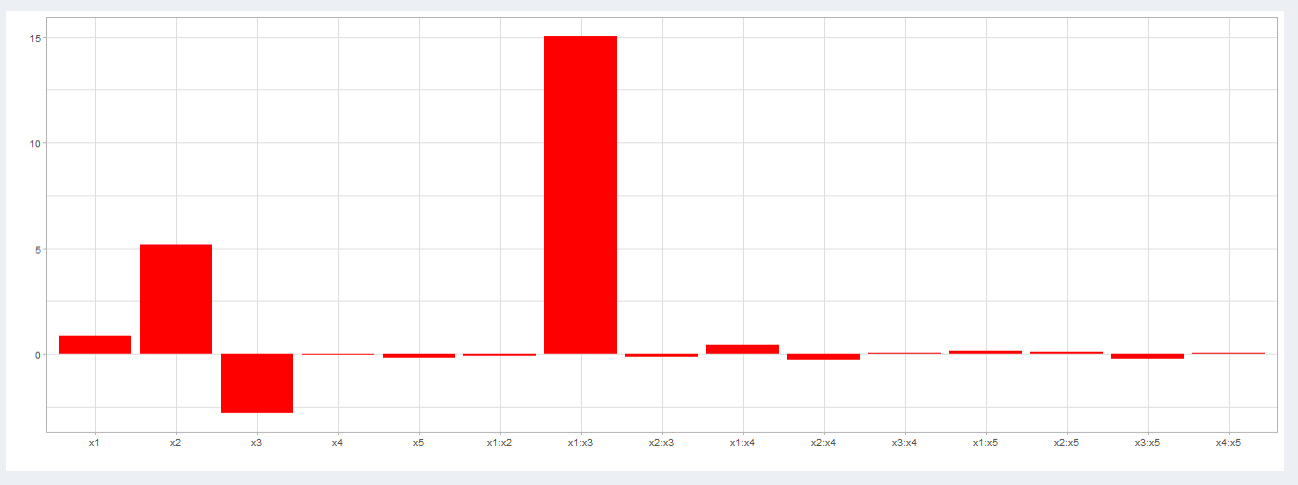
\includegraphics[width=1\linewidth]{Immagini/Fraz/12_Conf_ris5} 

}

\caption{Grafico dei coefficienti del modello frazionario $2^{5-1}_V$ }\label{fig:fz12}
\end{figure}

\newpage

Il disegno scelto ha risoluzione \(V\), ciò significa che i termini lineari sono confusi con le interazioni di ordine 4 e quindi posssiamo supporre che il valore di ciascun parametro si riferisca al termine lineare corrispondente (consideriamo trascurabili tutte le interazioni di ordine 4). E' possibile fare un ragionamento analogo per le interazioni di ordine 2 che si confondono con le interazioni di ordine 3. Supponendo che queste ultime siano trascurabili, possiamo dunque concludere che il valore di ciascun parametro di interazione si riferisca easclusivamente alle interazioni di ordine 2.

Se si volesse diminuire ulteriormente il numero di esperimenti, è possibile ricorrere ad un disegno frazionario \(2^{5-2}_{III}\), Tabella \ref{tab:Confris3}

\begin{table}

\caption{\label{tab:Confris3}Disegno frazionario $2^{5-2}_{III}$ (8 esperimenti) con risposte costruito dal modello supposto $y=x_1+5x_2-3x_3+15x_1x_3+\epsilon$}
\centering
\begin{tabular}[t]{rrrrrr}
\toprule
x1 & x2 & x3 & x4 & x5 & y\\
\midrule
-1 & -1 & -1 & 1 & 1 & 11.69\\
1 & -1 & -1 & -1 & -1 & -17.15\\
-1 & 1 & -1 & -1 & 1 & 20.62\\
1 & 1 & -1 & 1 & -1 & -6.44\\
-1 & -1 & 1 & 1 & -1 & -24.14\\
\addlinespace
1 & -1 & 1 & -1 & 1 & 7.07\\
-1 & 1 & 1 & -1 & -1 & -12.81\\
1 & 1 & 1 & 1 & 1 & 18.17\\
\bottomrule
\end{tabular}
\end{table}

Questo è un disegno di risoluzione \(III\), bisogna quindi fare molta attenzione alle confusioni Figura \ref{fig:fz13}

\begin{figure}[ht]

{\centering 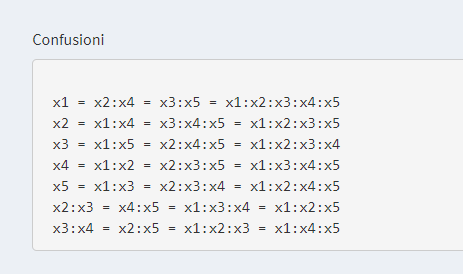
\includegraphics[width=1\linewidth]{Immagini/Fraz/13_Conf_ris3} 

}

\caption{Confusioni del disegno $2^{5-2}_{III}$}\label{fig:fz13}
\end{figure}

I termini lineari si confondono con le interazione di ordine 2. Come si vede dal grafico dei coefficienti Figura \ref{fig:fz14}

\begin{figure}[ht]

{\centering 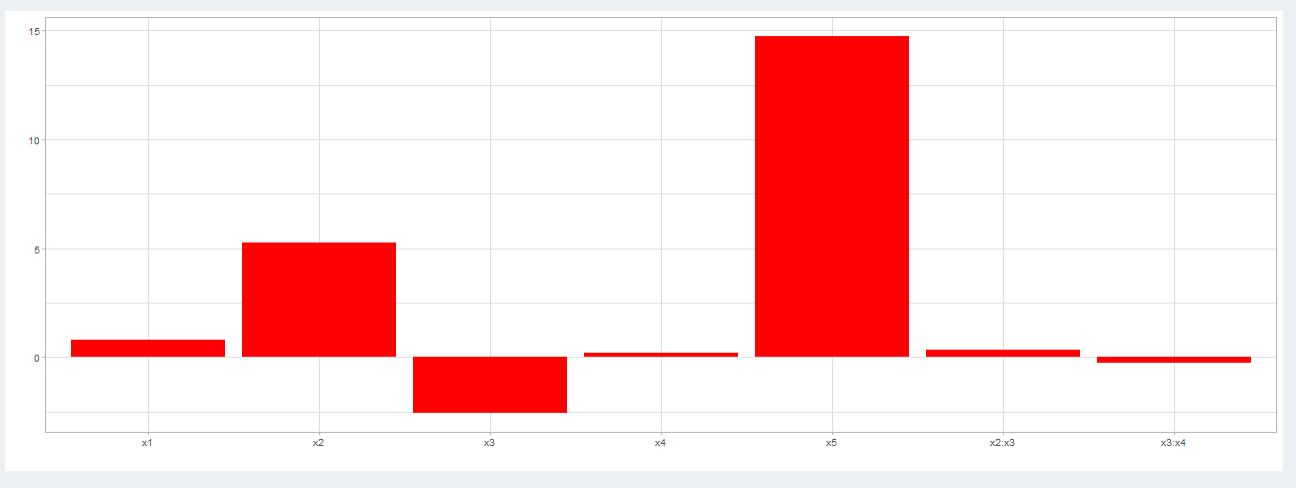
\includegraphics[width=1\linewidth]{Immagini/Fraz/14_Conf_ris3} 

}

\caption{Grafico dei coefficienti del disegno $2^{5-2}_{III}$}\label{fig:fz14}
\end{figure}

ad esempio il valore di \(x_5\) è circa 15, ma non siamo in grado di stabilire se è dovuto dal termine linerare \(x_5\), dal termine ``confuso'' \(x_1x_3\) (come in questo caso, ricordo la forma del modello \(y=x_1+5x_2-3x_3+15x_1x_3+\epsilon\)) o dalla combinazione di entrambi.

\hypertarget{esempio-studio-dei-fattori-dellestrazione-liquido-liquido}{%
\section{Esempio: studio dei fattori dell'estrazione liquido-liquido}\label{esempio-studio-dei-fattori-dellestrazione-liquido-liquido}}

Per meglio comprendere i disegni frazionari e l'utilizzo dell'applicativo in questi disegni consideriamo il seguente esempio.

Si vogliono studiare i seguenti 4 fattori:

\begin{itemize}
\item
  volume miscela solventi per estrazione
\item
  tempo di centrifuga dell'estratto
\item
  forza ionica del campione (quantità di NaCl da aggiungere)
\item
  tempo di estrazione
\end{itemize}

Definiamo innanzitutto il dominio sperimentale. Per ogni fattore determiniamo l'intervallo di valori compreso tra un massimo e un minimo entro i quali studiare il fenomeno, Tabella \ref{tab:fzliv}

\begin{table}

\caption{\label{tab:fzliv}Definizione dei livelli}
\centering
\begin{tabular}[t]{lcc}
\toprule
Fattori & -1 & +1\\
\midrule
vol. solvente & 10 & 40\\
t. centrifuga & 5 & 20\\
forza ionica & 1 & 5\\
t. estrazione & 1 & 5\\
\bottomrule
\end{tabular}
\end{table}

Il piano fattoriale completo prevede 16 esperimenti. L'impegno del laboratorio è considerato troppo oneroso. Si decide quindi di utilizzare un disegno frazionario \(2^{4-1}_{IV}\) per eseguire la metà degli esperimenti. Vedi Figura \ref{fig:fz4}

\begin{figure}[ht]

{\centering 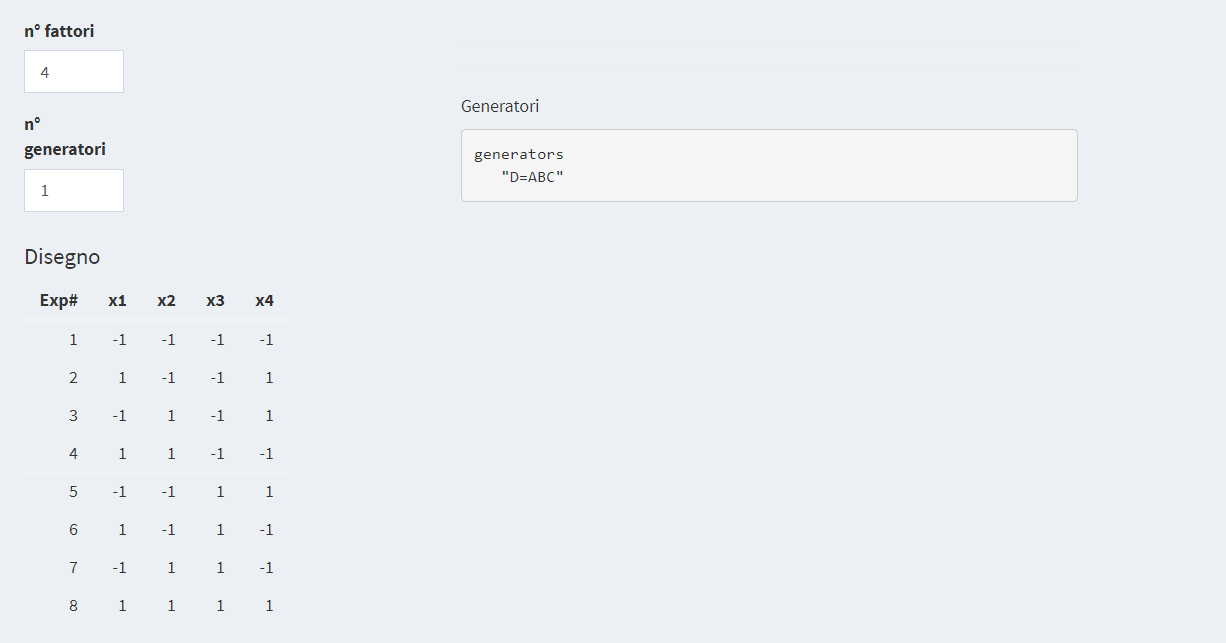
\includegraphics[width=1\linewidth]{Immagini/Fraz/04_esempio1} 

}

\caption{Disegno e generatore di  $2_{IV}^{4-1}$}\label{fig:fz4}
\end{figure}

Il piano sperimentale risulta quindi Tabella \ref{tab:piano}
\newpage

\begin{table}

\caption{\label{tab:piano}Piano sperimentale}
\centering
\begin{tabular}[t]{cccc}
\toprule
vol. solvente & t. centrifuga & forza ionica & t. estrazione\\
\midrule
10 & 5 & 1 & 1\\
40 & 5 & 1 & 5\\
10 & 20 & 1 & 5\\
40 & 20 & 1 & 1\\
10 & 5 & 5 & 5\\
\addlinespace
40 & 5 & 5 & 1\\
10 & 20 & 5 & 1\\
40 & 20 & 5 & 5\\
\bottomrule
\end{tabular}
\end{table}

Il modello e le ``confusioni'' sono dati in Figura \ref{fig:fz5}

\begin{figure}[ht]

{\centering 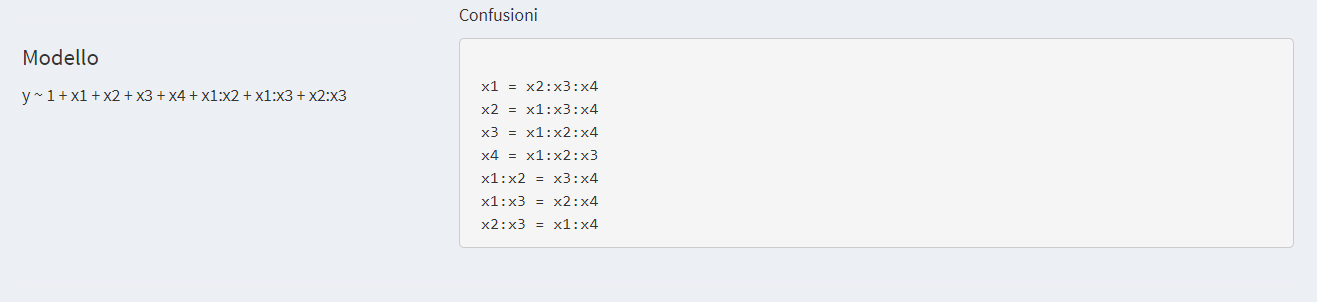
\includegraphics[width=1\linewidth]{Immagini/Fraz/05_esempio2} 

}

\caption{Modello e condusioni del frazionario di  $2_{IV}^{4-1}$}\label{fig:fz5}
\end{figure}

Il disegno è di risoluzione \(IV\) quindi, come si vede in Figura \ref{fig:fz5}, abbiamo ``confusione'' tra i termini lineari e le interazioni di ordine 3 e tra le coppie di interazioni di ordine 2.

Vengono quindi eseguiti, in ordine casuale, gli 8 esperimenti ottenendo per la risposta \emph{Resa} i seguenti valori, Tabella \ref{tab:fzpianorisp}

\begin{table}

\caption{\label{tab:fzpianorisp}Piano sperimentale $2_{IV}^{4-1}$ con risposte}
\centering
\begin{tabular}[t]{ccccc}
\toprule
vol. solvente & t. centrifuga & forza ionica & t. estrazione & Resa\\
\midrule
10 & 5 & 1 & 1 & 17\\
40 & 5 & 1 & 5 & 37.9\\
10 & 20 & 1 & 5 & 17\\
40 & 20 & 1 & 1 & 24.6\\
10 & 5 & 5 & 5 & 28.4\\
\addlinespace
40 & 5 & 5 & 1 & 22.7\\
10 & 20 & 5 & 1 & 30.3\\
40 & 20 & 5 & 5 & 36.3\\
\bottomrule
\end{tabular}
\end{table}

Inserendo nell'applicativo gli 8 valori della \emph{Resa} ottenuti (in ordine come in Tabella \ref{tab:fzpianorisp}, otteniamo la stima puntuale dei parametri Figura \ref{fig:fz6} e il relativo grafico Figura \ref{fig:fz7}.

\begin{figure}[ht]

{\centering 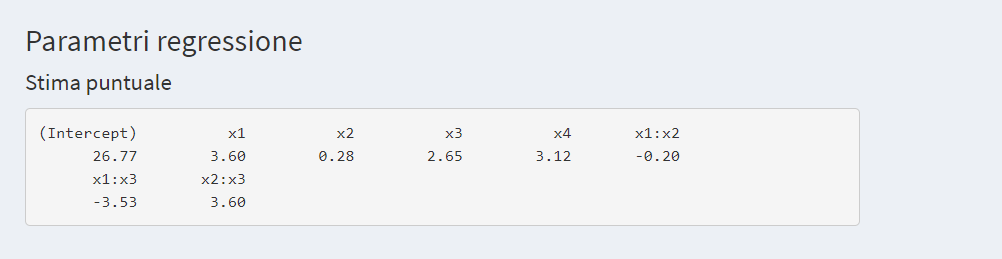
\includegraphics[width=1\linewidth]{Immagini/Fraz/06_parametri} 

}

\caption{Stima puntuale dei parametri}\label{fig:fz6}
\end{figure}

\begin{figure}[ht]

{\centering 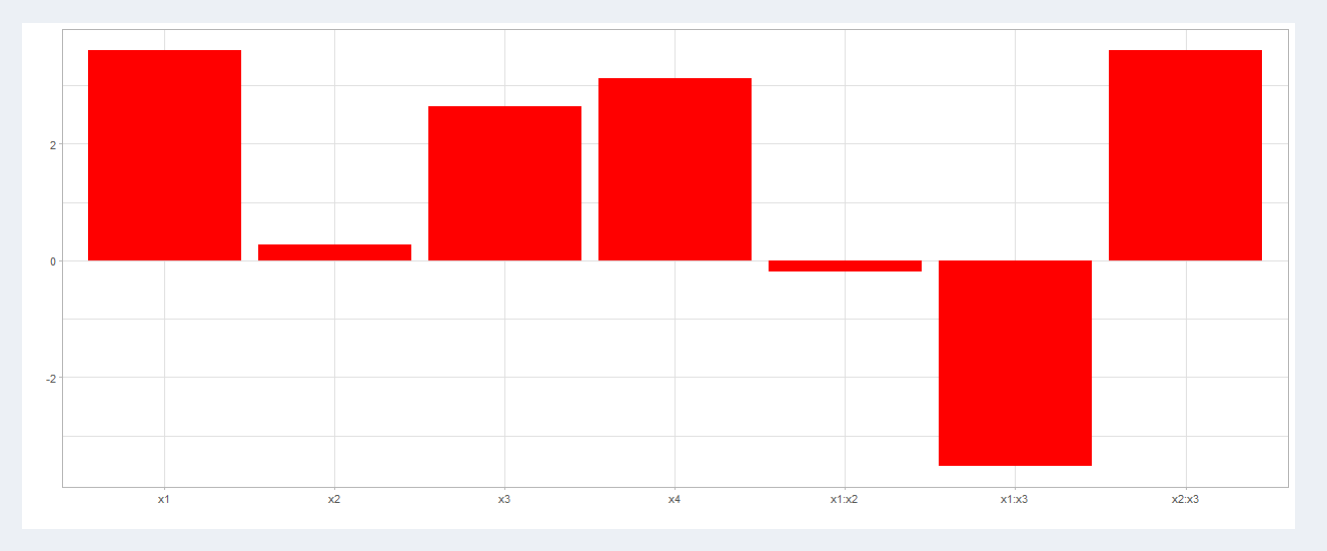
\includegraphics[width=1\linewidth]{Immagini/Fraz/07_graf_parametri} 

}

\caption{Grafico dell stima puntuale dei parametri}\label{fig:fz7}
\end{figure}

Ricordando le ``confusioni'' Figura \ref{fig:fz5} e che il disegno è di risoluzione \(IV\) abbiamo che il termini lineari sono ``confusi'' con le interazioni di ordine 3, possiamo quindi supporre che i valori dei parametri \(x_1,x_2,x_3\) e \(x_4\) si riferiscano ai termini linerari mentre rimangono le ``confusioni'' a coppie per le interazioni di ordine 2.\\
Il modello risulta quindi
\[
y=26.77+3.60x_1+0.28x_2+2.65x_3+3.12x_4-0.2(x_1x_2+x_3x_4)-3.53(x_1x_3+x_2x_4)+3.60(x_1x_4+x_2x_3)
\]

Il fattore \(x_2\) ha coefficiente piccolo e non sembra importante, mentre gli altri tre termini lineari lo sono sicuramente.\\
Quindi si può sostenere l'ipotesi che le interazioni confuse siano dovute ai termini diversi da \(x_2\).\\
Questa osservazione è di fatto risultata coerente con il dato sperimentale osservato secondo cui il tempo di centrifuga non ha alcun effetto sulla resa di estrazione perché il livello più basso scelto è già più che sufficiente per rompere l'emulsione creata dopo la miscelazione delle fasi del solvente di estrazione e del campione.
Tali conclusioni sono confermate dal piano \(2^4\) poi condotto a termine.

Il modello finale semplificato quindi è

\[
y=26.77+3.60x_1+2.65x_3+3.12x_4-0.2x_3x_4-3.53x_1x_3+3.60x_1x_4
\]

Per convalidare il modello sono state eseguite misure indipendenti nel punto test \((1-1,-1,-1,-1)\). Inserendo le rese osservate \(17.2,16.9,17.0,16.8\) nell'apposita casella dell'applicativo si ottiene Figura \ref{fig:fz8}

\begin{figure}[ht]

{\centering 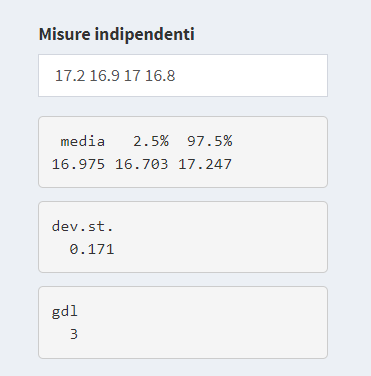
\includegraphics[width=1\linewidth]{Immagini/Fraz/08_mis_ind} 

}

\caption{Misure indipendenti nel punto test}\label{fig:fz8}
\end{figure}

La risposta predetta nel punto test e gli estremi dell'intervallo di confidenza costruito con la stima di \(\sigma\) ottenuta con le 4 misure indipendenti sono dati in Figura \ref{fig:fz9}.

\begin{figure}[ht]

{\centering 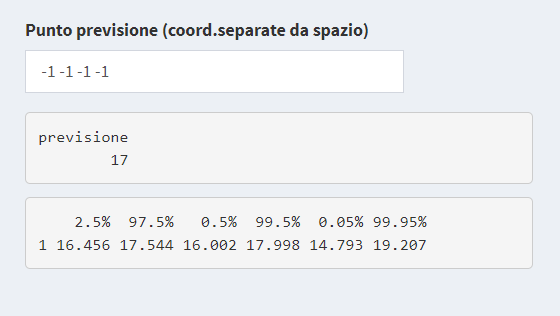
\includegraphics[width=1\linewidth]{Immagini/Fraz/09_prev} 

}

\caption{Previsione nel punto test e estremi dell'intervallo di confidenza}\label{fig:fz9}
\end{figure}

Il modello è convalidato statisticamente e può quindi essere usato per esplorare in modo attendibile il dominio delle risposte, Figura \ref{fig:fz10}

\begin{figure}[ht]

{\centering 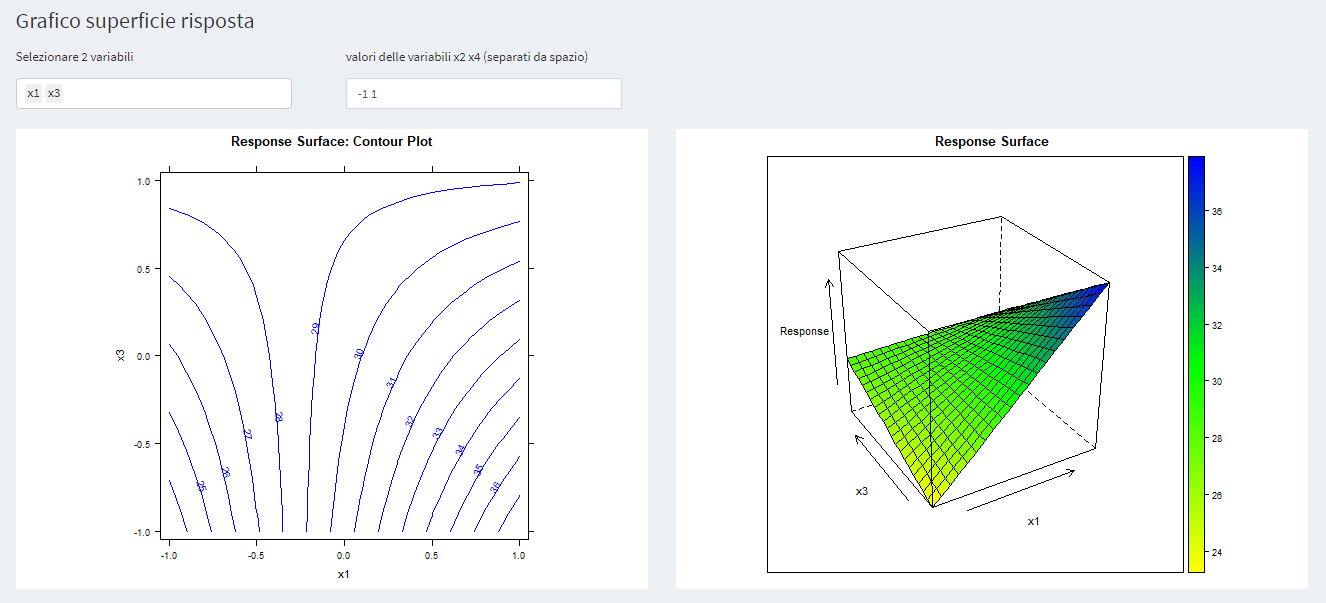
\includegraphics[width=1\linewidth]{Immagini/Fraz/10_sup_risp} 

}

\caption{Grafico della superficie di risposta}\label{fig:fz10}
\end{figure}

\backmatter

  \bibliography{book.bib}

\addcontentsline{toc}{chapter}{Bibliografia}

\end{document}
